%# -*- coding: utf-8-unix -*-
%%==================================================
%% conclusion.tex for SJTUThesis
%% Encoding: UTF-8
%%==================================================

\chapter{引言}
\label{chap:introduction}
光学文本识别是派生自光学文字识别(Optical Character Recognition,OCR)的一个活跃的课题,在图像中提取其中蕴含的丰富的文本信息在数字化的今天变得愈发的重要。
从公路电子摄像头抓拍提取车牌,到历史档案和公司文件的数字化存储,我们能在生活中发现大量的 OCR 应用场景。
不像人脑能够从图像中轻易地捕获并识别出文字,机器往往没有足够的智能来准确地理解和识别图像中的文本信息。
所以尽管该课题已经被广大学者研究了几十年,构建一套能够匹敌自然人的能力的文本识别系统依然是一个开放且富有挑战性的任务。
并且,由于语言的种类之多,其语法之复杂,再加之字体和风格,甚至于光学图像的噪声和形变,这些原因造成了光学文本识别变成了一个复杂的问题。
囿于上述挑战和需求,大量的科学界和工业界的学者投身于改进光学文本识别系统。
如今,一套完整的光学文本识别系统涉及到相当广泛的计算机科学子学科。

光学文字识别可以追溯到计算机的发展之前,最早的 OCR 系统不是计算机而是一套机械设备,虽然它不仅识别速度很低,而且识别精度也很低。
在 1951 年,M. Sheppard 发明了能够识别音乐符号和单词的机器 GISMO,虽然它只能识别 23 种字符,这套系统甚至还可以复制手写文本的纸张。
随后,J. Rainbow 在 1954 年发明了一个能够识别大写字母的机器,然而它的速度依然很慢,一分钟只能识别出一个字。
这些早期的 OCR 系统因其错误率和识别速度饱受诟病,所以在 60 年代和 70 年代很少有人研究 OCR,唯一的研究兴趣来源于政府部门及大型企业(例如银行,报纸和航空公司)。
因为识别的复杂性,人们开始寻求 OCR 字体的标准化,以简化 OCR 的实现复杂度。
于是在 1970 年,ANSI 和 EMCA 发起了 OCRA 和 OCRB,它们提供了相对而言可被接受的识别率。

\begin{figure}[h!]
	\centering
	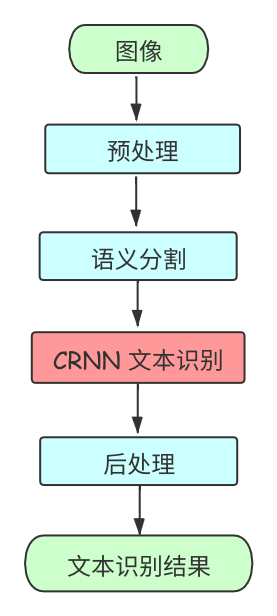
\includegraphics[width=0.25\textwidth]{figure/resources/OCR_system.png}
	\caption{\textbf{光学文本识别系统概览}\label{ocr_system_overall}}
\end{figure}

在过去的三十多年里,学术界已经在 OCR 领域打下了扎实的基础。
这推动了文档图像识别(document image analysis,DIA),多语言,手写体,任意字体 OCR 等就技术的兴起与发展。
随着以深度学习为代表的技术在图像和自然语言处理领域取得的突破性成就,近年来,学者们开始尝试将深度学习有关技术应用于 OCR 系统中 \cite{CRNN,MFCNN,SEE,CTPN},这些技术主要集中在文本的检测和识别中。
一套完整的光学文本识别主要包括:

\begin{itemize}
	\item \textbf{预处理}:预处理操作用于提高图片质量及其感兴趣区域。
	\item \textbf{语义结构分割}:虽然语义结构分割可以算是预处理的一部分,不过由于所使用的方法较复杂,且对后面的文本识别有着明显的影响,所以我们将该部分单独作为一个组件。
	\item \textbf{文本识别}:对预处理完的含有文本的图像块进行文本识别,有两种级别:字符级识别和字符序列级别。
	\item \textbf{后处理}:虽然目前 OCR 系统(包括端到端的字符序列识别)已经能够到达较高精度,然而它们识别出来的结果依然不可避免的含有一些错误的字符,亦或是缺字多字。后处理就是使用语义模型等复杂模型或字典查询等简单规则对识别结果进行进一步的修正和增强。
\end{itemize}

图\ref{ocr_system_overall}展示了光学文本识别系统的概览,其中文本识别模块是必须的,输入为图像,而其他三个蓝色的模块(预处理,语义结构分割和后处理)都是可选的。
在复杂和具有大量噪声的场景文本识别任务中,这些最新的 OCR 技术已经取得了积极的进展。
然而,上述工作重点仍然在计算机视觉,将图像分类和物体检测等技术应用于 OCR 任务中。
相对于常规的计算机视觉任务,OCR 所面临的数据不仅有丰富图像信息,而图像中的文本也有丰富的语义信息。
例如,在含有大块文本的图片中,这些文本往往不是杂乱无章的,而是一段自然语言,例如一篇论文,一份公司财报,亦或是一篇手写信。
在自然语言中,一个单词或者字在某处出现的概率,与它所处的上下文有相当大的关系。
并且,OCR 识别的结果中,往往容易出现个别字的识别误差,这是因为神经网络模型不能很完美地泛化到图像中有的所有字。
常见的 OCR 识别误差包括:

\begin{enumerate}[(1)]
	\item \textbf{替换错误}:错误地把一个字识别成另外一个字,例如两个字形状非常类似。
	\item \textbf{冗余错误}:识别出了额外的字,该误差可能来自将噪声错误识别为字,或者从一个字的各个部分识别除了多个字,同时在 CTC 解码过程中也容易出现该错误。
	\item \textbf{遗漏错误}:识别结果中遗漏了部分字,该误差可能来自图像中某些字噪声或者形变比较严重,也有可能是 OCR 系统没有很好的泛化到这些图形上。
\end{enumerate}

这些识别误差一般是在后处理模块中进行检测和修正。
在识别误差中,虽然某些字形状非常类似,但是在特定的上下文下,人类通过语义分析很容易去判断和修正这样的错误。
同样的,这些 OCR 的识别误差会造成整段文本中出现明显的离群文字。
对于文本的语义分析,在自然语言处理领域,我们可以使用统计语言模型或者基于深度学习的语言模型来建模每个字在这段自然语言文本中的概率。
当前光学文本识别的研究主要着眼于提高速度和精度的同时,很少有研究使用自然语言处理的技术去理解和修正文本识别内容的语义正确性。
因此,基于这些发现,本文主要研究和实现使用语义分析来提高 OCR 系统的精确度和性能。

本学位论文主要的研究内容和贡献如下:

\begin{enumerate}[(1)]
	\item \textbf{构建了一个大规模文本识别数据集。} \\
	为了获取足够的训练样本,我们使用来源各种领域的新闻作为语料库,基于 70 余中中文字体,以及多种数据增强技术,创建了一个含有 160 多万样本,由 6000 多个常用汉字、标点符号和英文字母构成的数据集。
	\item \textbf{研究并实现了基于 ConvS2S 的 OCR 后处理模块。} \\
	我们受到文献\cite{NLPCC}将机器翻译模型 ConvS2S 用于中文语法错误修正的启发,将 ConvS2S 应用于 OCR 识别错误的语义修正。
	\item \textbf{研究并实现了基于 BERT 和 Transformer 的 OCR 后处理模块。} \\
	我们发现带有 OCR 识别错误的结果与正确的结果的关系类似于 BERT 中的带掩码的语言模型任务,基于此发现,我们将大规模语料库中预训练的 BERT 语言模型和在机器翻译领域取得重大进步的 Transformer 的模型结合在了一起,用作后处理模块对 OCR 模型的识别结果进行修正。
	\item \textbf{与其他已有研究成果进行对比实验。} \\
	我们将我们提出的方法与不带后处理模块的 CRNN 以及基于 $n$-gram 的后处理模块进行对比,并分析了这些已有方法的特点和不足之处。
\end{enumerate}

在第\ref{chap:related_work}章介绍有关的研究现状后,为了更好的方便读者,我们将在第\ref{chap:prerequisite}章中介绍预备知识,随后在第\ref{chap:cs2s}章和第\ref{chap:bert_nmt}中我们将详细地提出我们的方法和网络结构。
并且在第\ref{chap:experiments}章中,我们将构造我们的数据集和实验环境,并与其他已有的研究进行对比,验证我们提出的模型的性能。
最后,我们总结我们提出的模型的特点并提出展望。

\chapter{基于深度学习的光学文本识别研究现状}
\label{chap:related_work}
本章节中我们主要对文本识别系统的框架中每一个组件的研究现状逐一介绍,希望借此为读者提供一个对光学文本识别系统较全面的认识。
首先文本识别系统的框架我们已经在第\ref{chap:introduction}章做了简要介绍,本章节后续内容将围绕该框架展开。
值得一提的是,本章所覆盖的方法只不过是本方向众多论文的冰山一角,难免遗漏了许多有代表性的文章。


\section{预处理}
对于来自扫描仪的图像,一般来说图像质量是比较高的,而许多时候,图像的来源不止扫描仪,还有许多来源于普通的光学相机。
并且,这些来源于光学相机的图像往往有许多噪声和扭曲,甚至有些是在较差的环境下拍摄所得。
为了解决这些图像质量问题以增强图像质量,许多预处理方法被提出。
这些操作一般使用一些比较简单的操作来对所有图像做统一的预处理,有偏斜消除,基线识别,噪声消除,还有灰度化。
还有一些复杂一点的模型也会被用到,例如文本方向识别。

\begin{figure}[h!]
	\centering
	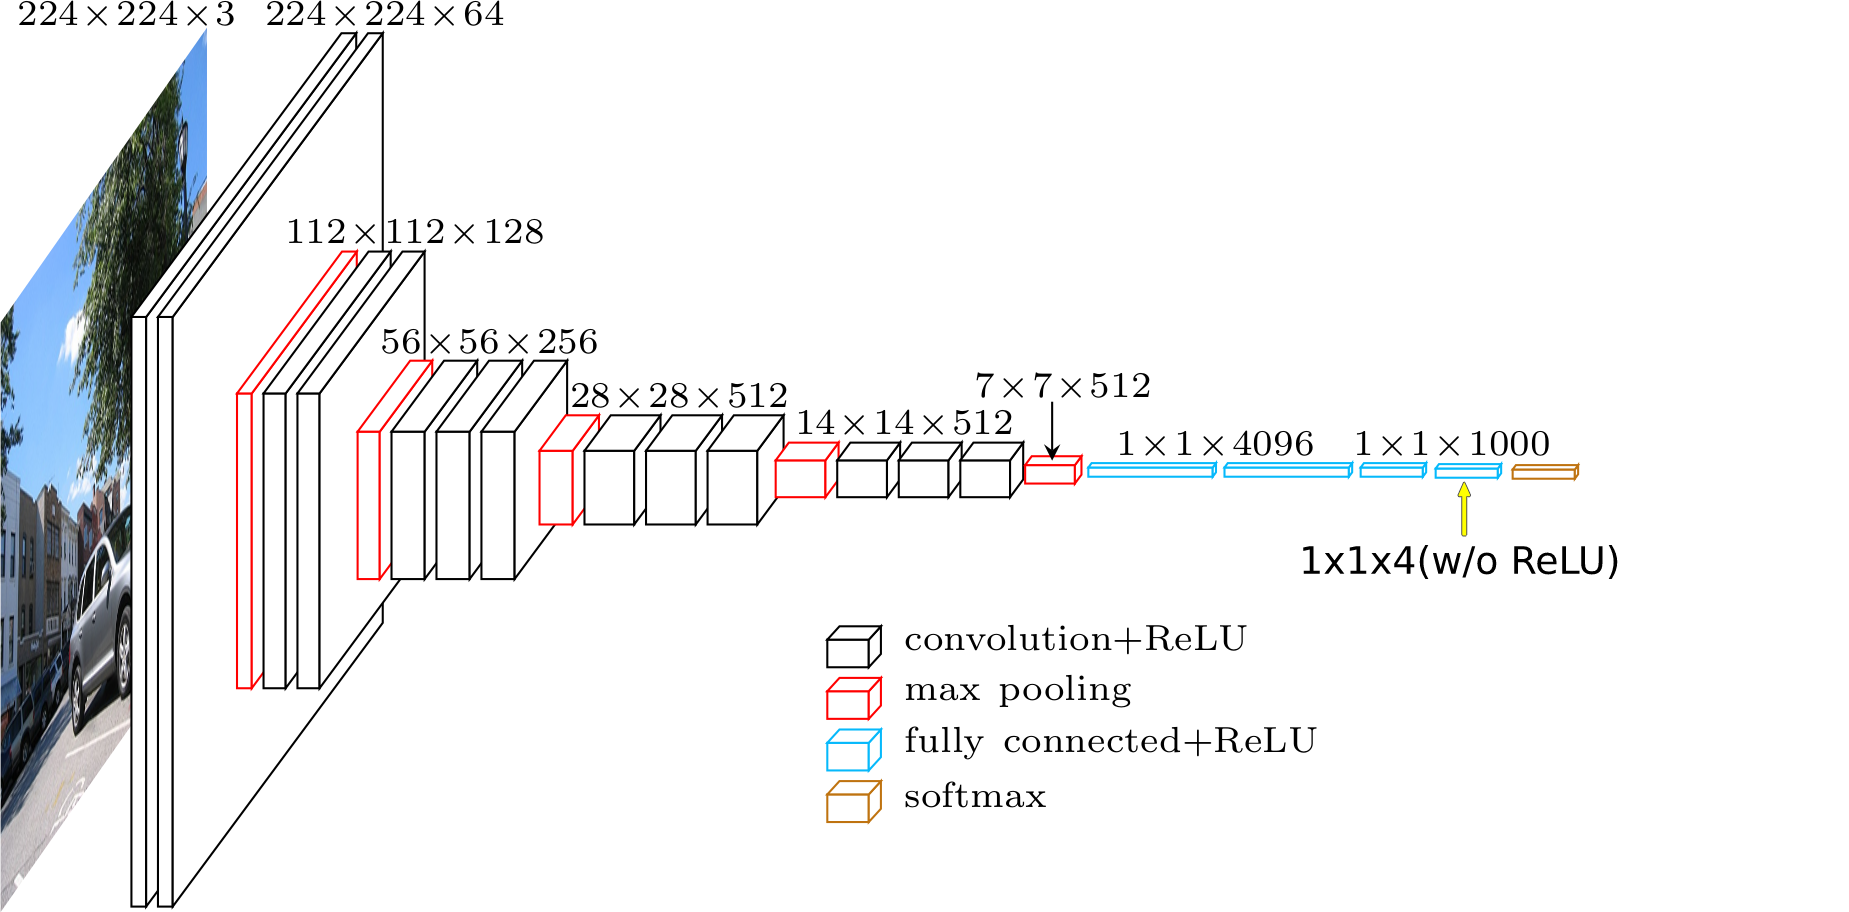
\includegraphics[width=0.75\textwidth]{figure/resources/vgg16_text_angle.png}
	\caption{\textbf{VGG16 文本方向识别模型}\label{vgg16_text_angle}}
\end{figure}

文本识别任务中图像中往往会含有多种方向的文字(0、90、180、270度),所以许多文本识别系统会在预处理的时候进行文字方向识别。
本节介绍一个使用 VGG16\cite{vgg} (项目地址\footnote{Github 仓库:\url{https://github.com/xiaofengShi/CHINESE-OCR}})进行文本方向的例子。

因为检测结果只有四种文字方向,而原始的 VGG16 是 $1000$ 分类,所以我们需要修改 VGG16 的最后一层全连接层(dense layer)为四分类,经过修改的 VGG16 的整体架构图见图\ref{vgg16_text_angle}。
主要的修改就是在大小为 $1000$ 的全连接层与 softmax 层之间加入一个没有激活单元的大小为 $4$ 的全连接层。

\section{语义结构分割}
传统的 OCR 系统往往以字符为单位进行,也就是每一个图像块有且只有一个字符。而随着深度学习的高速发展,许多学者开始转向使用表达能力更加强的深度学习技术来进行端到端的文本识别(也就是说,直接从整个图像中识别整段文本)。
所以,语义分割的单位也可以分为字符和文本块。

虽然 YOLO 论文中的数据集本身不是用于文本分割的模型,不过我们可以很简单的将 YOLO 用于文本语义分割任务。
按照引用数量和刊物等级,我们介绍以下两种方法:YOLOv3\cite{yolov3},CTPN\cite{CTPN}。

\begin{table}[!hpt]
	\caption[]{\textbf{语义结构分割有关论文}}
	\label{tab:preprocessing_papers}
	\centering
	\begin{tabular}{c c c c}
		\hline
		方法 & 引用数 & 发表刊物 & 发表时间 \\ [0.5ex] 
		\hline
		YOLO & 7042 & CVPR & 2016 \\
		CTPN & 318 & ECCV & 2016 \\
		\hline
	\end{tabular}
\end{table}

\subsection{YOLO}
YOLO 系列论文由于其高效的速度及可观的识别结果连续几年作为物体识别领域的业界标杆,虽然 YOLO 最初不是用于文本语义结构识别,不过可以很方便地将 YOLO 迁移到文本语义识别领域。

首先我们简要介绍一下 YOLO\cite{YOLO}。
相对于许多组合多个神经网络来进行物体检查论文,YOLO 首先提出把物体识别变为一个回归任务,使用单个网络直接输入图片并输出所有识别出的物体的有界框(bounding boxes)及类别等信息。
虽然 YOLO 对比当时的最新研究(state-of-the-art),精确度低一些,当时 YOLO 的高效及强大的泛化能力是它的亮点。

YOLO 的大致工作流为:首先把图片分成 $S \times S$ 的网格,如果有要识别的物体落在该网格上,则该网格能够反映它识别了该物体。
每个网格预测 $B$ 个有界框及其置信度,这些置信度反映了该框中是否有物体的可能性大小,定义为 $Pr(Object)*IOU^{\texttt{truth}}_{\texttt{pred}}$,因为作者希望如果框内没有物体,则置信度为 $0$否则作者希望置信度为预测框和实际的 IOU(intersection over union)。
每一个有界框含有五个预测项:$x,y,w,h$ 以及置信度,其中 $x,y$ 表示框中心相对于该网格的距离,$w,h$则表示框的宽度和长度相对于整个图片大小的比值,并且它们都会归一化到 0 到 1 的范围。
其中一个网格预测 $C$ 个条件类别概率:$Pr(Class_i|Object)$,这些概率是在该有界框含有物体的条件之下的,值得一提的是 YOLO 没有在同一个网格中为每个有界框预测所有类别的概率。
测试的时候每个框的类别置信度就是这个条件类别概率乘以每个框的置信度:$Pr(Class_i|Object)*Pr(Object)*IOU^{\texttt{truth}}_{\texttt{pred}} = Pr(Class_i)*IOU^{\texttt{truth}}_{\texttt{pred}}$。
所以最后我们需要做回归的就是一个大小为$S \times S \times (B * 5 + C)$ 的张量。

\begin{figure}[h!]
	\centering
	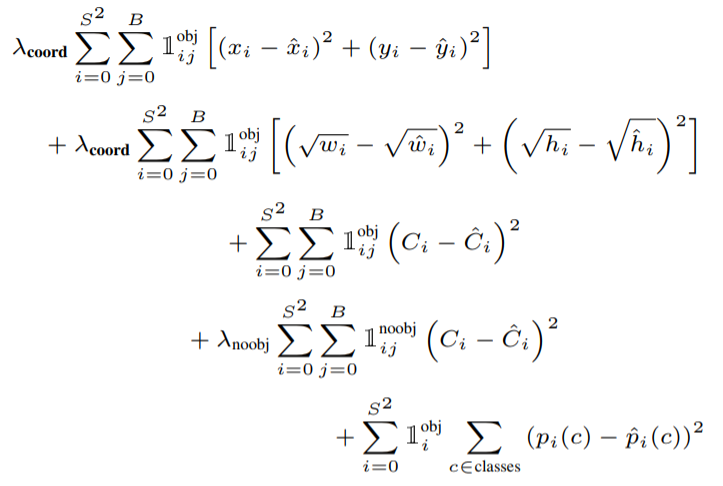
\includegraphics[width=0.5\textwidth]{figure/resources/YOLO_loss.png}
	\caption{\textbf{YOLO 损失函数}\label{YOLO_loss}}
\end{figure}

最后,YOLO 使用基于方差和(sum-squared error)的损失函数见图\ref{YOLO_loss}。
其中,$\lambda_{\text{coord}} = 5, \lambda_{\text{noobj} = 0.5}$ 用来增加有界框的坐标预测的损失值并减少有界框中没有物体时的置信度的损失值。
$\mathbb{I}_i^{\texttt{obj}}$ 表示如果物体在网格 $i$ 中则为 $1$ 否则为 $0$。
$\mathbb{I}^{\texttt{obj}}_{ij}$ 表示网格 $i$ 的有界框 $j$ 是有对应的物体(因为不一定所有 $B$ 个框都有物体,很多时候是所有都没有或者只有一个框。
可以很容易看出大部分损失函数只针对有物体的时候。

\subsection{CTPN}
Connectionist Text Proposal Network (CTPN) 直接在卷积层定位文本,这解决了之前许多基于字符检测的自底向上的方法的主要局限。
CTPN 将文本识别问题转化为定位细粒度的文本部件(text proposals)组成的序列的问题,并且作者还开发了一种锚点回归机制(anchor regression mechanism)为每一个文本部件预测垂直位置和是否是文本的置信度,同时在网络内使用循环神经网络来将这些序列文本部件优雅地连接起来。
所以,CTPN 是一个可以处理多语系(multi-lingual)和多尺度(multi-scale)文本的,统一的,端到端的,可训练模型。

因为文本不像一般物体具有封闭的轮廓和明显的中心,文本一般指单词或整段文本,所以整段文本其实是由稀疏的更小的单位(单词,字符,句子)组成,如果直接把文本块当做物体识别,很容易导致识别系统把文本快的部分(例如单词的一部分)当做整个物体。
所以,很容易想到将文本行作为一个细粒度的文本部件组成的序列。
文本部件可以理解为文本行的一小部分。
每个文本部件一般包含一个或多个笔画,一个字符的一部分,或者多个字符。
作者认为在固定更难预测的水平位置的情况下,只预测每个文本部件的竖直位置会更加的准确且简单(因为缩小了搜索空间)。

\section{文本识别模型}
本节中我们主要分析基于深度学习的文本识别模型,这类模型一般有两种,一种是结合文本语义分割和文本识别的模型,一种是将按照文本行语义分割和规整化之后的图像作为输入的文本识别模型。
一般来说,文本语义分割和文本识别所需要的样本数量和样本特点不尽相同。
前者主要需要在样本中分布着足够多不同形状位置的文本块,以期能够涵盖大部分应用场景并识别出这种图片中的文本快和文本行。
而后者主要需要样本中含有足够多的字符以及各种噪声,这些噪声包括扭曲,模糊,非文本内容等等。
固然将文本分割和文本识别拆成两个独立的模型会不可避免的的造成一些不必要的冗余开销,不过这有利于按照各自的特点准备不同的数据集进行训练,也有利于在模块之间添加额外的后处理模块。
综上,我们主要介绍后者,也就是不考虑文本语义分割的文本识别模型,其中主要以 Baoguang Shi 等提出的卷积循环神经网络(CRNN)\cite{CRNN}为代表进行介绍。
CRNN 是 2017 年发表在 TPAMI 的一篇期刊论文,其引用数目前已有 $583$ 之多,足见起有效性及影响力。
CRNN 是一个集成了特征提取,序列建模和转录(transcription)于一体的端到端的可训练神经网络,并且借助 RNN 的能力,CRNN 很自然地拥有处理任意长度序列的能力,它不需要耦合任何预定义的词库(lexicon)。
在本文中,我们将 CRNN 作为文本识别的骨干(backbone)网络。

\subsection{CRNN}
\label{crnn}

\begin{figure}[h!]
	\centering
	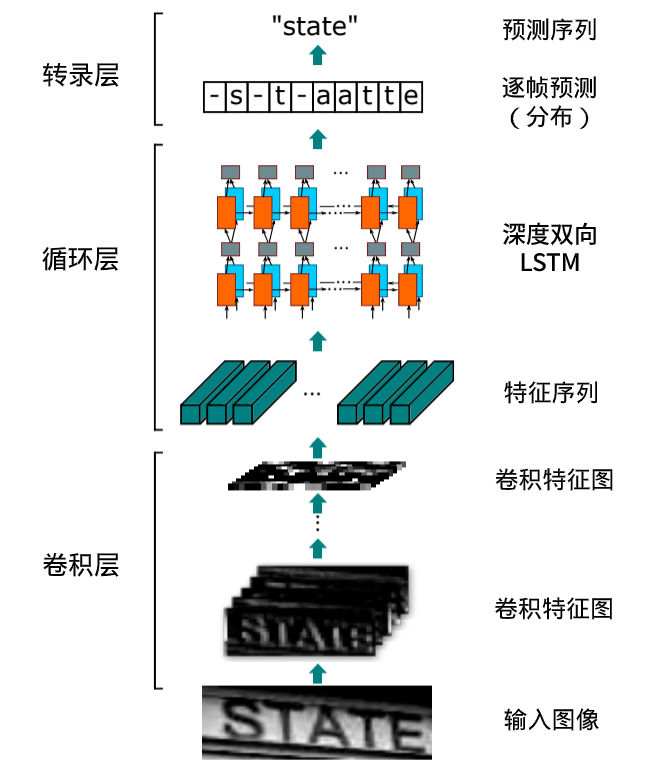
\includegraphics[width=0.5\textwidth]{figure/resources/CRNN_arch.png}
	\caption{\textbf{CRNN 网络结构}\label{CRNN_arch}}
\end{figure}

CRNN 的整体网络结构可见图\ref{CRNN_arch},它输入为固定大小的图像,自底向上主要由三个部分组成:卷积层,循环层和转录层。
卷积层用于从每一张图像中自动提取特征序列,而循环神经网络则用于将特征序列中转化为预测,转录层用于将每一帧的 RNN 预测翻译为标签序列。
虽然 CRNN 由多种神经网络组成,但是它可以使用一个损失函数进行联合训练。

接着,对于特征图(feature maps),从左往右按列生成特征序列中特征向量,也就是说第 $i$ 个特征向量是所有特征图的第 $i$ 列串接而成。
其中每一列的宽度被固定为一个像素。
由于 CNN 的感受野(receptive field)的缘故,特征图的每一列对应原始图片的一个矩形区域,并且从左往右的顺序也是一一对应的。
CRNN 首先使用卷积操作和池化操作将二维图像转化为一位特征序列,序列中每一个元素为图像中对应感受野的特征向量。
随后 RNN 负责对序列进行处理,学习每一帧的上下文的识别特征以修正结果,例如识别“il”的时候,通过对比它们的高度差别要比单个的识别它们更加简单。
此外,RNN 可以将误差梯度信息方向传播到输入,也就是说,传播到卷积层。
这样带来的好处是可以联合训练卷积层和循环层。

转录层则是要将 RNN 的逐帧预测输出转化为标签的概率分布。
转录有分为两种:无需词典(lexicon-free transcription)和基于词典的(lexicon-based transcription),词典就是一组固定的标签序列。
无需词典模式就是说预测结果不需要借助任何词典,而词典模式就是寻找概率最大的并且在词典中的标签序列。
因为中文不像英文单词由许多字母组成,中文的词大多与字符一致,并且词之前没有严格的分隔符(例如英文中的空格用作单词之间的分隔符)。
类似韩语和日语,中文作为一种语标语言(logographic language),字符种类相当庞大(一万左右个字符),而英语只有 26 种字母。
所以词典模式在中文文本识别中,用处不太明显,并且英文单词识别时也容易发现单词不在词典的情况。
CRNN 使用 CTC (Connectionist Temporal Classification ,连通时域分类)\cite{CTC}层作为条件概率。
简单来说,CTC 作为一种用于序列到序列(Seqeucen-to-Sequence,Seq2Seq)的单调对齐手段,它可以将序列中的连续的相同字符收缩成一个字符,并且自动跳过一种特殊字符——空字符(blank token)。
CTC 作为一种简单的技术可以将序列转换为不同长度(更短的)的序列,以达到 Seq2Seq 的目的。
空字符在 CRNN 应用场景中代表该感知野所在区域没有识别结果,例如本来就没有字符,或者字符残缺。
而连续的重复字符可以被视作卷积核滑动过程中,多个感知野都覆盖到并识别出了了同一个字符。
定义输入序列为 $\bm{y} = y_1, \cdots, y_T$,并且每个 $y_t \in \mathbb{R}^{|L|}$,其中 $L$ 是含有空字符的字典。
CTC 映射函数描述为 $\mathcal{B}: \mathbb{R}^{|L|} \rightarrow \mathbb{R}^{<|L}$.
例如 $\mathcal{B}(\text{--hh-e-l-ll-oo--}) = \text{hello}$,其中 “-” 表示空字符。
最终输出 $\bm{l}$ 关于 $\bm{y}$ 的条件概率定义为所有能够通过 $\mathcal{B}$ 映射到 $\bm{l}$ 的所有路径 $\bm{\pi}$ 之和:

\begin{equation}
	p(\bm{l} | \bm{y}) = \sum_{\bm{\pi}: \mathcal{B}(\bm{\pi}) = \bm{l}} p(\bm{\pi} | \bm{y})
\end{equation}
其中 $p(\bm{\pi} | \bm{y}) = \prod_{t=1}^T y_{\pi_t}^t$,$y_{\pi_t}^t$ 表示时间步 $t$ 时标签为 $\pi_t$ 的概率。

\begin{table}[!hpt]
	\caption[]{\textbf{本文使用的 CRNN 网络架构}\label{tab:crnn}}
	\small
	\centering
	\begin{tabular}{cc}
		\hline
		\textbf{类型} & \textbf{配置} \\ [0.5ex] 
		\hline
		输入 & 灰度图,固定高度 $32$,宽度 $w$ \\
		卷积层 $1$ & 通道数 $64$,卷积核 $(3,3)$,步长 $(1,1)$,填充 $(1,1)$ \\
		卷积层 $2$ & 通道数 $128$,卷积核 $(3,3)$,步长 $(1,1)$,填充 $(1,1)$ \\
		批次归一化层(Batch Normalization) & - \\
		最大池层 $1$ & 卷积核 $(2,2)$,步长 $(2,2)$,填充 $(1,1)$ \\
		卷积层 $3$ & 通道数 $256$,卷积核 $(3,3)$,步长 $(1,1)$,填充 $(1,1)$ \\
		卷积层 $4$ & 通道数 $512$,卷积核 $(3,3)$,步长 $(1,1)$,填充 $(1,1)$ \\
		批次归一化层(Batch Normalization) & - \\
		最大池层 $2$ & 卷积核 $(2,2)$,步长 $(2,2)$,填充 $(1,1)$ \\
		瓶颈层 $1$ & 通道数 $512$,卷积核 $(3,3)$,步长 $(1,1)$,填充 $(1,1)$ \\
		瓶颈层 $2$ & 通道数 $512$,卷积核 $(3,3)$,步长 $(1,1)$,填充 $(1,1)$ \\
		批次归一化层(Batch Normalization) & - \\
		最大池层 $3$ & 卷积核 $(2,2)$,步长 $(2,1)$,填充 $(1,1)$ \\
		瓶颈层 $3$ & 通道数 $512$,卷积核 $(4,1)$,步长 $(1,1)$,填充 $(0,0)$ \\
		输出 & 通道数 $512$,高度 $1$, 宽度 $w / 4 - 1$ \\ 
		\hline
	\end{tabular}
\end{table}

\begin{figure}[h!]
	\centering
	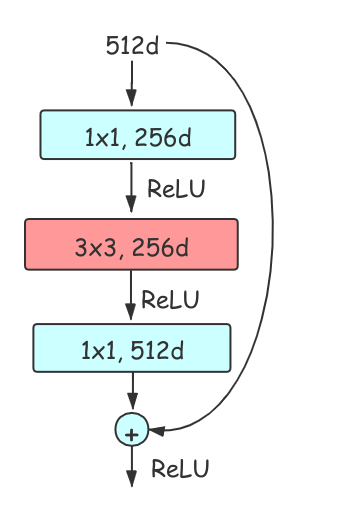
\includegraphics[width=0.25\textwidth]{figure/resources/bottleneck.png}
	\caption{\textbf{残差连接和瓶颈层的结构}\label{bottleneck}}
\end{figure}

相对于 CRNN 原文所描述的神经网络结构,本文适当的调整了网络结构,并使用了额外的残差连接以及瓶颈设计(bottleneck)\cite{ResNet},并且将激活函数调整为 Leaky ReLU\cite{leaky_relu}。
我们实现的 CRNN 网络的具体配置可见表\ref{tab:crnn},其中我们将瓶颈层 $1$ 的输入与瓶颈层 $2$ 的输出进行残差连接。
残差连接和瓶颈层的结构见图\ref{bottleneck},将输入和输入直接相连的便是残差连接。
瓶颈层的设计有助于设计更加深的网络,其中使用的 $1 \times 1$ 卷积运算速度极快,并且有助于降低通道间的冗余。
具体的网络架构在表\ref{tab:crnn}中详细列出,该网络因为最大池和卷积核大小的原因,会将输入宽度缩小 $4$ 倍多。
批归一化处理(batch normalization)\cite{batch_norm}用于加速收敛,其原理主要是将神经网络的隐藏层输出在同一批次同不同样本间的协方差偏移归一化。

\section{基于语义分析的后处理}
虽然现有的 OCR 系统已经有很高的精确度和较强的范化能力了,但是仍然不可避免地含有个别错误,比如错字,缺字多字。
同时,NLP 领域已经发展地比较成熟了,我们可以使用 NLP 的技术来对 OCR系统识别出的结果已经后处理,精细化和处理少数错误。
但是相对于英语法语这样的字母语言,中文不仅词汇量大,而且由于中文书写的复杂性,中文拼写错误纠正更加难以解决。
例如”今天的天气很好“很容易被错误识别为”令天的天气很好“。
再加之中文没有明显的分词界限,不同的分词也许代表完全不一样的语义,中文文字识别的后处理因此变得更加棘手。
拼写检查大致分为基于规则的和基于统计的方法,显然基于规则的方法会更有局限性,而统计方法具有很好的鲁棒性。
所以综上所述,造成中文文本系统的后处理任务的困难之处主要在于:
\begin{enumerate}[(1)]
	\item 汉字的词汇量大,且含有大量相似字,同义字,再加之中文书写和语法的复杂性。
	\item 中文没有明显的分词界限,不同的分词也许代表完全不一样的语义。
	\item 文本在不同工作环境下有明显特征(例如发票),但是缺少拼写检查有关的大型数据集,大部分数据只有图片和文本的对应关系。
\end{enumerate}

本章中,我们主要简要介绍一个基于机器学习的方法,简称为基于SMT(Statistical Machine Translation)的方法\cite{post_SMT}和基于 $n$-gram 语言模型和迷惑集的方法\cite{huang2014chinese,mei2016statistical}。

\subsection{基于 SMT 的方法}
该论文基于短语统计机器翻译(phrasal statistical machine translation)框架来进行中文拼写错误检测和修正,该方法结合了基于规则的方法和基于统计的方法,使用统计模型来解决基于规则的方法忽视上下文的问题。
大致的思路主要分为以下三个部分:
\begin{enumerate}[(1)]
	\item 中文句子被分段为词。
	\item 检测模块用于检测和标记可能有拼写错误的词。
	\item 在错误修正阶段,使用 SMT 模型来将含有拼写错误的句子转化为正确的。
\end{enumerate}

使用分词来减小搜索空间和错误率,不过中文分词常常会出现过分词(over-segmented )现象,SMT 模型则可用于解决该问题。
例如“除了要有超世之才,也要有堅定的意志”可能被过分词为:“除了/要/有/超世/之/才/,/也/要/有/堅定/的/意
志”。
扩充词典也是一种解决方案。
因为拼写错误往往导致一串单字出现在分词结果中,所以所有由单字导出的 $n$-grams将考虑作为候选错误词(candidates)。
该方法有个潜在的局限性就是,如果词组不在词典里面,则它们会被视作拼写错误。

找出拼写错误的列表后,SMT 尝试将句子翻译为正确的形式。
当给定一个拼写错误的词,首先通过将字符替换为相似的字,一次替换一个,来生成所有的正确假设。
例如对于“氣份”一词,部分正确假设为:汽份,泣份,
器份, 契份,
企份, 憩份,
氣分, 氣忿,
氣憤, 氣糞,
氣奮, 氣氛。
这些翻译假设将使用词典来验证(修剪)。
翻译概率定义为:
\begin{equation}
tp = \log_{10} \left(\frac{freq(trans)}{freq(trans) - freq(condi)}\right)*\gamma
\end{equation}

解码器用于单调的(也就是不改变原来语序)翻译语法错误,翻译模型使用GIZA++,语言模型使用 SRILM。

\begin{table}[!hpt]
	\caption[]{\textbf{SMT 翻译样例}}
	\label{tab:smt_tanslation}
	\centering
	\begin{tabular}{c c c c}
		\hline
		\textbf{翻译} & \textbf{频率} & \textbf{语言模型概率} & \textbf{tp} \\ [0.5ex] 
		\hline
		氣憤 & 48 & -4.96 & -1.20 \\
		氣氛 & 473 & -3.22 & -1.11 \\[1ex] 
		\hline
	\end{tabular}
\end{table}

\subsection{基于 $n$-gram 统计特征和迷惑集的方法}
\label{n_gram}
该方法主要基于 $n$-gram 统计特征和迷惑集对 OCR 识别结果或者其他带有拼写错误的文本进行修正。
$n$-gram 作为一种简单有效的统计语言模型,被广泛用于衡量给定单词序列的品质以及预测下一个将出现的单词。
因此,$n$-gram 统计特征可以用于检测和修正带有错误的文本。
同时,迷惑集作为一种基于专家经验的硬规则手段,为识别错误提供了丰富的潜在候选选择。
例如,对于“\textbf{丁}”字,跟它形状类似的字有 “\textbf{订 钉 叮 盯 打}”,这个候选迷惑集中的字有可能被 OCR 系统错误识别成候选集中的其他字。

\begin{figure}[h!]
	\centering
	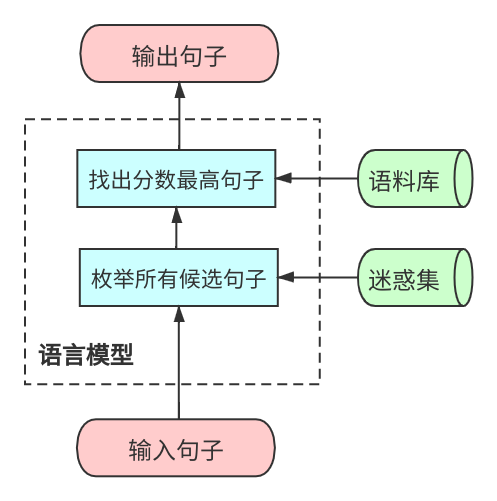
\includegraphics[width=0.5\textwidth]{figure/resources/CSC.png}
	\caption{\textbf{基于 $n$-gram 统计特征和迷惑集的后处理方法流程图}\label{CSC}}
\end{figure}

该方法完整的流程图如图\ref{CSC} 所示,它主要包含三个组件:

\begin{enumerate}[(1)]
	\item 首先对于给定的输入句子,该后处理系统首先为每一个字符按照迷惑集提供候选字集合。
	\item 对于句子中的每个字符,后处理系统会枚举使用每一个候选字替换它,进而产生候选句。
	\item 通过 $n$-gram 语言模型,为每一个候选句打分,最后分数最好的候选句就被选择为最终的输出句子。
\end{enumerate}

对于 $n$-gram 语言模型,给定一个中文字符序列 $C = c_1, \cdots, c_L$,我们定义第 $t$ 词 $c_t$ 在给定上文下的概率分布为:

\begin{align}
	\label{ngram}
	P(c_t | c_1, \cdots, c_{t-1}) &= \frac{P(c_{t-n+1}, \cdots, c_{t-1}, c_t)}{P(c_{t-n+1}, \cdots c_{t-1})} \nonumber \\
	&= \frac{N(c_{t-n+1}, \cdots, c_{t-1}, c_t)}{N(c_{t-n+1}, \cdots c_{t-1})}
\end{align}

也就是说,$n$-gram 限定词 $c_t$ 的上文感知野大小为 $n-1$。
其中 $P(c_{t-n+1}, \cdots, c_{t-1}, c_t)$ 只需要通过 $n$ 元组 $(c_{t-n+1}, \cdots, c_{t-1}, c_t)$ 在整个语料库出现的次数除以归一化因子即可。
同理 $P(c_{t-n+1}, \cdots c_{t-1})$ 等于 $n-1$ 元组 $(c_{t-n+1}, \cdots c_{t-1})$ 在整个语料库出现的频率。
所以,对于整个句子 $C$ 的语言模型概率我们只需要将每个词的上文概率累乘即可得到该联合概率:

\begin{equation}
	P(C) = \prod_{t=1}^L P(c_t | c_1, \cdots, c_{t-1})
\end{equation}

常见的 $n$ 的取值为 $2 \sim 7$,随着 $n$ 的增加 $n$-gram 的数量会呈现指数级别的暴增,同时会造成严重的稀疏性问题。
也就是说,会存在大量的 $n$-gram 的出现次数直接为 $0$。
不失一般性地,我们在这里适用 $3$-gram。

因为枚举所有候选句子并选择分数最高的句子的复杂度极高,所以我们可以使用动态规划对其进行优化。
首先假定 $c_t$ 对应的迷惑集为 $V[i]$,迷惑集的第 $j$ 和元素为 $V[i][j]$。
我们将分数最高的后卷句定义为 $dp[i][j][k]$,并且第 $i-1$ 个字符为 $V[i-1][j]$,$V[i][k]$ 就是第 $i$ 个字符。
因为 $3$-gram 只依赖 前面两个字符,所以我们就可以通过动态规划算法得到状态转移函数:

\begin{equation}
	s = (V[i-1][j], V[i][k], V[i+1][l]) \\
	dp[i+1][k][l] = \max(dp[i+1][k][l], dp[i][j][k] * P(s))
\end{equation}
其中 $P(s)$ 便是三元组的 $3$-gram 概率。

这样,通过动态规划,枚举所有候选句子并选择分数最高的句子的复杂度就就降低到 $\mathcal{O}(LN^3)$,其中 $N$ 为迷惑集的大小。

其次,为了解决 $n$-gram 的稀疏性问题,文献\cite{huang2014chinese}对公式\ref{ngram}加入拉普拉斯平滑来解决概率的稀疏性问题。
首先我们简要介绍一下 Laplace 平滑,这个技术最初用于将类别数据平滑化。
对于一个参数为 $\bm{\theta} = (\theta_1, \cdots, \theta_d)$ 的多项式分布我们采样 $N$ 次,得到 $\bm{x} = (x_1, \cdots, c_d)$,参数的平滑版本的估计为:

\begin{equation}
	\hat{theta}_i = \frac{x_i + \alpha}{N + \alpha d}, i=1,\dots,d
\end{equation}
其中 $\alpha > 0$ 为平滑参数。

作为一种收缩估计,Laplace 平滑的估计结果为经验估计 $x_i / N$ 和均值概率 $1/d$ 之间。
这样,采用 Laplace 平滑的 $n$-gram 概率的变种为:

\begin{align}
	P_{\text{smooth}}(c_t | c_1, \cdots, c_{t-1}) &= \frac{P_{\text{smooth}}(c_{t-n+1}, \cdots, c_{t-1}, c_t)}{P_{\text{smooth}}(c_{t-n+1}, \cdots c_{t-1})} \nonumber \\
	&= \frac{N(c_{t-n+1}, \cdots, c_{t-1}, c_t) + \alpha}{N(c_{t-n+1}, \cdots c_{t-1}) + \alpha d}
\end{align}

\section{本章小结}
本章节系统全面的介绍了文本识别系统的一般结构和组成成分,本文的研究方向主要集中与后处理部分。

\chapter{预备知识}
\label{chap:prerequisite}

\section{Transformer}
在以往的基于卷积神经网络的序列到序列模型中,因为感知野的缘故,要将输入和输出中任意两个位置的信号联系起来需要的卷积操作数和两个位置的距离成正比。
具体来所,在 ConvS2S\cite{cs2s} 模型中,比例为线性,在 ByteNet\cite{ByteNet} 中,该比例为对数。
这使得这些模型更难学习到远距离依赖,在 Transformer 架构\cite{transformer}中,要学习任意距离之间的依赖都只需要常数级别的复杂度。
Transformer 完全抛弃了卷积操作和序列对齐的循环(recurrent)操作,它的核心在于自注意力(self-attention)机制的使用。
自注意力机制是一种只通过同一个序列的不同位置的之间的关系来作为权重以获得序列的表示的一种注意力机制。
同样的,Transformer 的总体架构也是编码器-解码器架构。
对于给定输入序列的符号表示为 $(x_1, \cdots, x_n)$,编码器首先将其转化为连续表示的序列 $\bm{z} = (z_1, \cdots, z_n)$。
对于给定的 $\bm{z}$,解码器生成输出序列 $(y_1, \cdots, y_m)$,并且每次只生成一个元素。
也就是说,为了产生长度为 $m$ 的输出序列,解码器需要执行 $m$ 次。

\begin{figure}[h!]
	\centering
	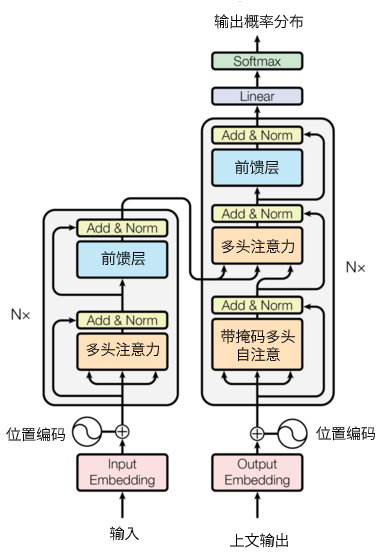
\includegraphics[width=0.5\textwidth]{figure/resources/transformer.png}
	\caption{\textbf{Transformer 网络}\label{transformer}}
\end{figure}

Transformer 的完整网络架构在图\ref{transformer}中展示,它的解码器和编码器均采用堆叠的自注意力和全连接层。
在原文中,编码栈和解码栈均由六层相同的层组成。其中,一个编码层由两个子层组成:多头自注意力层和前馈全连接层。
每一个子层的输出均采用层归一化技术(layer norm)和残差连接:$y = \text{LayerNorm}(x + \text{SubLayer}(x))$,其中 $\text{SubLayer}$ 表示子层。
而对于解码栈,一个解码层由三个子层组成:带掩码的多头自注意力层、多头自注意力层以及前馈全连接层。
首先我们定义什么是注意力机制:注意力函数可以被描述为将一个查询和一组键值对映射到输出,输出就是通过对查询和这些键之间的运算产生的权重对这些值加权求和而产生的。
每一个值的权重由这个查询和对应的键运算产生。

具体来说,Transformer 使用的是一种叫做“缩放点乘注意力”的注意力机制,输入为 $n_q$ 个维度为 $d_k$ 的查询 $Q \in \mathbb{R}^{n_q \times d_k}$,一组含有 $n_p$ 的键值对:维度为 $d_k$ 的键 $K \in \mathbb{R}^{n_p \times d_k}$,维度为 $d_v$ 的值 $V \in \mathbb{R}^{n_p \times d_k}$。
注意力输出为:

\begin{equation}
	\text{Attention} (Q, K, V) = \text{softmax}(\frac{QK^\top}{\sqrt{d_k}}) V
\end{equation}
其中对于 $X \in \mathbb{R}^{n_q \times n_p}$, softmax 函数用于将其中的列向量归一化为概率分布,定义为:

\begin{equation}
	\text{softmax}(X)_{ij} = \frac{\exp(X_{ij})}{\sum_j \exp(X_{ij})}
\end{equation}

上述公式中缩放因子 $\sqrt{d_k}$ 是作用是,当 $d_k$ 很大的时候,容易倒是点乘后的结果的绝对值非常大,进而导致它们 softmax 归一化的时候处于梯度极小的位置,这样非常不利于梯度传播。
对于带掩码的情况,softmax 的输入会首先由一个形状相同的 0-1 矩阵指定值为 0 的位置被掩饰(mask)为 $-\infty$,这样经过 softmax 之后它们对应的概率值就变味了 $0$,这样可以使得加权累加的时候忽略部分键对值的影响(即权重为 0)。
为了使得自注意力也能像卷积神经网络中通过大量的通道来表示不同的特征以增加模型的表示空间,Transformer 引入多头自注意力机制:通过将 $Q,K,V$ 映射到不同的子空间进而学习不同的自注意力输出,最后在将这些输出联合起来:

\begin{equation}
	\text{MultiHead}(Q,K,V) = \text{Concat}(\text{head}_1,\cdots,\text{head}_h) W_O
\end{equation}
其中 $\text{head}_i = \text{Attention}(Q W_i^Q, KW_i^K, VW_i^V)$,$W_i^Q \in \mathbb{R}^{d_m \times d_k}, W_i^K \in \mathbb{R}^{d_m \times d_k}, W_i^V \in \mathbb{R}^{d_m \times d_v}, W^O \in \mathbb{R}^{d_m \times d_m}$, 并且限定 $d_k = d_v = d_m / h$,函数 $\text{Concat}(\cdot)$ 用于将其中的元素的最后一维连接起来(将 h 个 $d_v$ 维连成 $d_m$ 维)。

多头自注意力层的输入为 $Q,K,V$。而按照输入的不同以及是否使用掩码,Transformer 中使用的多头自注意力网络有三种:

\begin{enumerate}[(1)]
	\item 在编码层,$Q,K,V$ 均来自同一个序列,长度为 $n_s$,也就是来只上一层的输出。这样序列中的每一个位置都可以跟输入中的所有位置进行联动。
	\item 在解码层的带掩码的自注意力子层,其 $Q,K,V$ 均来自同一个输入,也就是已解码的序列,用于获得当前的上文信息。注意区别于编码层,解码的时候我们只能看到上文而不能获取下文,例如,目标句子为 “我爱自然语言处理”,当前已经解码的内容为“我爱自然语”,而我们无法知道后续的“言处理”。在带掩码的自注意力子层中,对于长度 $n_t$ 的输出句子序列,共有 $n_t$ 个查询,第 $i$ 个查询代表获取第 $i$ 个位置的上文,也就是我们需要屏蔽掉 $i$ 及以后的内容。这便是掩码的作用,所以掩码矩阵使用上三角矩阵即可。我们需要类似编码层,解码层的带掩码的自注意力子层的输入便是上一层编码层的输出。
	\item 在解码层中的另外一个自注意力子层,该子层用于将编码层和解码层结合起来。查询来自于在解码层的带掩码的自注意力子层的输出 $Q \in \mathbb{R}^{n_s \times d_m}$,而值和键均来自于编码层最后一层的输出 $Q = K \in \mathbb{R}^{n_s \times d_m}$。这样最后产生的序列形状为 $n_t \times d_m$,其长度便是目标序列的长度,并且第 $i$ 个位置上的特征向量表示输出序列的第 $i$ 个位置。
\end{enumerate}

编码器和解码器中的每一层都有一个简单的逐位前馈层(position-wise feed-forward networks),它用于将特征转换到新的表示空间并减少特征向量不同维度之间的冗余。
其形式化表示为:

\begin{equation}
	\text{FFN}(\bm{x}) = \text{ReLU}(\bm{x} \bm{W}_1^{l} + \bm{b}_1^{l}) \bm{W}_2^{l} + \bm{b}_2^{l}
\end{equation}
其中 $\bm{W}_1^{l} \in \mathbb{R}^{d_m \times d_f}, \bm{W}_2^{l} \in \mathbb{R}^{d_f \times d_m}$,$\text{ReLU}(x) = \max(0, x)$ 为一种简单的非线性激活单元。并且值得一提的是,每一层的逐位前馈层的参数都是不一样的。

在 Transformer 应用于自然语言处理任务时(例如机器翻译),我们首先需要对这些离散的单词(或者字母,词片段等)转换到连续域的嵌入(embedding)表示。
输入和上文的词嵌入向量是共享的,并且词嵌入会乘以 $\sqrt{d_m}$,$d_m$ 为词嵌入的维度。
因为 Transformer 中不含有循环单元也不含有卷积单元,为了当模型能够利用序列中的顺序信息,模型必须在输入序列中插入相对或绝对位置信息。
为了达到这一目的,模型在编码层和解码层的第一层输入之间引入位置编码(positional encodings)。
位置编码为三角函数族,这些函数的频率不同:

\begin{equation}
	\text{PE}(pos, 2i) = \sin(pos / 10000^{2i/d_m}) \\
	\text{PE}(pos, 2i+1) = \cos(pos / 10000^{2i/d_m})
\end{equation}
其中 $pos$ 表示位置,$i$ 表示维度。
这使得每一个维度都是不一样的正弦函数,波长从 $2\pi$ 到 $10000 \cdot 2\pi$。
选用这样的函数的目的是,论文作者假设这样能够让模型轻松学到相对位置信息,因为对于任意固定的偏移量$k$,$PE(pos+k)$中能够表示为$PE(pos)$的一个线性函数。
另外,在原嵌入加上位置编码之后,还会使用 Dropout \cite{dropout}技术来避免过拟合,丢弃率为 $0.1$。
位置编码函数示例可以参见图\ref{position_encodings}。

\begin{figure}[h!]
	\centering
	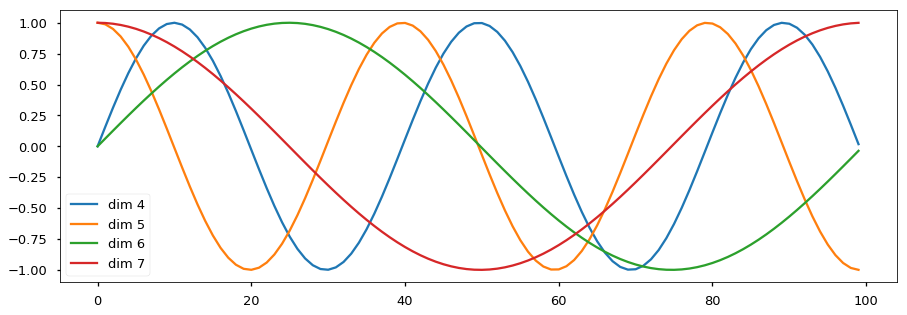
\includegraphics[width=0.8\textwidth]{figure/resources/position_encodings.png}
	\caption{\textbf{位置编码函数示例}\label{position_encodings}}
\end{figure}

除了上述核心内容,论文也用了许多技巧。
假如每次解码的时候只选择概率最高的那个结果,那么如果该结果是错误的,则后续结果均会受到这个错误的上文的结果的影响。
所以在解码过程中,每一次解码并不只产生一个结果(例如机器翻译中的一个单词),而是按照概率分布保存概率较大的前 $k$ 个结果作为候选假设,并且在下一轮解码的时候,将这 $k$ 个候选假设参与计算并同理继续选择 $k$ 个概率最大的候选结果。
每条候选路径的概率为其中每一个元素的概率的乘积。
这种解码方式称为束搜索(beam search)。
其次,传统的交叉熵损失函数的准则概率分布为独热分布,这样会造成模型预测的结果也倾向于独热分布,也就是说如果模型预测错误,其它候选结果的概率都会变得很小。
这样不利于束搜索,所以 Transformer 使用平滑标签的交叉熵损失函数,即准则分布在正确的标签上的概率不是 1 而是一个较大值(例如 0.9),而其他标签平均分配其余概率。
此外,词片段\cite{subword}的使用用有助于解决词模型英文等语言中存在的单词不在词典的情况。
优化器采用 Adam\cite{adam},并且超参数设置为 $\beta_1 = 0.9, \beta_2=0.98, \epsilon=10^{-9}$。
学习率采用逆方差的变种:$lr = d_m^{-0.5} \times \min(s^{-0.5}, s \times w^{-1.5})$,其中 $s$ 为当前的更新布,$w$ 为预热步数,默认为 $4000$。
也就是说,学习率会在前 $4000$ 步缓慢爬升,之后按照步数的逆方差来缓慢降低。

\section{BERT 预训练语言模型}
基于 Transformer 的双向编码表示是一种设计用于海量无标签文本中预训练深度双向表示的神经网络,它能够结合所有层中左边和右边两种方向的上下文。
它的一个优点就是基于 BERT 预训练模型,只需要加一个输出层就可以微调到大量的下游任务,例如问答、命名实体识别、语言推导和阅读理解等,不需要额外的针对不同人物进行重新设计网络结构。
在微调至下游任务时,BERT 首先从预训练模型中初始化其参数,然后所有的可训练参数将会使用针对下游任务的新的目标函数和数据标签进行微调。

BERT 的模型架构类似于 Transformer 中的编码层, 其基准模型采用 $L=12$ 层自注意力单元,头数设置为 $A=12$,并且隐藏特征维度为 $H=768$,逐位前馈层的中间维度为 $4H = 3072$,总参数数量为 $340$M。
虽然 OpenAI GPT\cite{GPT} 也是基于 Transformer 架构的无监督学习预训练模型,不过 GPT 采用的是类似于 Transformer 解码器中使用的带掩码的自注意力层,所以属于单向模型,每个位置上的元素只能感知到上文的内容而无法感知到下文的内容。
然而,下文的内容同样非常重要,例如在问答任务上,很多时候答案往往出现在下文中。
并且,不管是单个句子还是像问答任务中的问题和答案句子对,BERT 均能无歧义地表示它们。
在 BERT 中,句子不是一般意义上的以断句符号结尾的句子,而是一段连续文本的任意区块。
每个句子的开头为叫做分类符(classificatin token)的特殊标识符 \texttt{[CLS]},模型的最终输出中该位置可用于表示分类任务结果。
对于句子对,BERT 首先将他们打包成单个句子,通过在他们中间插入特殊标识符 \texttt{[SEP]}。
其次,每个输入单元,包括这些特殊标识符,都会被加上一个可训练嵌入,用于表示它是否输入第一个句子抑或是第二个句子。

在预训练 BERT 的时候,其核心内容就是它的目标函数,与传统的基于从左到右或者从右到左的语言模型作为训练任务不同的是,BERT 使用两个无监督任务作为目标函数:

\begin{enumerate}[(1)]
	\item \textbf{带掩码的语言模型(Masked LM)}:为了训练深度双向表示,我们只需要简单的从输入序列中随机隐藏掉部分单元,然后通过这些隐藏元素的上下来预测它们。具体来说,隐藏比例为 $15\%$,损失函数为交叉熵。因为下游任务中不会出现特殊标识符\texttt{[MASK]},所以 BERT 采用广义的掩码来修正:要被掩码的词有$80\%$的可能被替换为\texttt{[MASK]},而有 $10\%$的可能替换为随机的词,还有另外 $10\%$的可能不变。不过这种隐藏方式容易造成,相关性极大的一组词可能被同时隐藏,例如如果我们需要预测被掩码的句子“[MASK] [MASK] is a city.”中的第二个词,原始句子为“New York is a city.”,因为前面两个词的关联性极大,所以这样的情况会显著的影响模型的性能。基于这个问题,XLNet \cite{cite}提出了叫做重排列语言模型的目标函数用于修正该问题。
	\item \textbf{下一句预测(NSP)}:许多下游任务的输入为句子对,例如问答任务,所以 BERT 特意为句子对准备了一个二分类任务。具体来说,有 $50\%$ 的可能性,输入的句子对 $A$ 和 $B$ 不属于上一句话和下一句话的关系,$B$ 有可能来自于任意预料中的任意句子。NSP 就是判断 $B$ 是否是 $A$ 的下一句。不过按照 XLNet \cite{xlnet}中的研究表明,因为 $B$ 有 $50\%$ 的可能性来自于另外的语料库的句子,这样导致 NSP 任务相当于两个任务:判断是否属于同一文档的上下句关系的任务,以及判读是否属于同一文档的任务。而这两个任务的难度明显是不成正比的,明显前者要比后者难。所以训练过程中很有可能导致模型只学习到了后者的任务并且也能得到了不错的训练误差。
\end{enumerate}

虽然 BERT 预训练模型取得了很不错的结果,不过其模型比较庞大,如果将其用作新模型的一小部分,会导致大量的额外资源消耗。
ALBERT\cite{albert} 基于这个问题以及 NSP 的问题。
提出了一个轻量级的 BERT 模型,其中所有层全部共享相同的参数,这样极大的减小了模型大小和显存占用,有利于创建更加深的 BERT 模型,不过不足之处是训练和测试时间变化不大。
并且不同于 Transformer 中嵌入向量的维度和自注意力的维度相同,ALBERT 提出使用大的嵌入向量维度,然后使用较小的自注意力维度,这样同样能够减少模型参数,只需要在嵌入层输出和自注意力输入之间增加一个全连接层即可。
对于 NSP 问题,ALBERT 任务 NSP 任务在问答任务中确实发挥着重要的作用,所以提出句子顺序任务(SOP)替换掉 NSP 任务。句子顺序任务同样是而分类任务,只不过负例为 $B$ 跟 $A$ 的次序对掉。 

\section{Dropout}
深度神经网络作为一种强有力的机器学习技术,因其庞大的参数规模,以及非常深的非线性复合函数,它们能够表达相当复杂的假设空间。
然而,在此类网络中,过拟合是一种常见但非常严重的问题。
因为庞大的神经网络需要大量的运算资源,通过结果多个不同的庞大的神经网络的预测结果作为测试结果往往又是不切实际的。
Dropout\cite{dropout} 技术由 Nitish Srivastava 等人提出,作为一种正则化手段在缓解模型过拟合上有着明显的效果。
它的主要原理非常简单:在训练阶段随机移走部分神经单元的输出,这样有利于减少共生单元过多的情况。
具体来说,在训练过程中,dropout 会从 Bernoulli 分布产生一个掩码向量,并用于隐藏层的输出,随机取消部分单元的输出:

\begin{equation}
	d_i \sim \text{Bernoulli}(1 - p_{\text{drop}}) \\
	\hat{\bm{h}}^{(t)} = \bm{d} \odot \bm{h}^{(t)}
\end{equation}
其中 $\odot$ 为逐位乘法,对于输出为 $\bm{h}^{(t)} \in \mathbb{R}^{D_h}$ 的隐藏层 $t$,掩码向量为 $\bm{d} \in \{0,1\}^{D_h}$。
在测试时,我们需要使用神经网络的所有单元。
并且如果在测试时使用 dropout,这会导致结果变得非常不稳定,因为就算是相同的样本,因为 Bernoulli 分布的缘故,都有可能得到不同的测试结果。
因为 dropout 会显著地改变网络的输出量纲(可以理解为数学期望),所以我们需要在测试时对其进行修正。
因为对于 dropout 的输出 $\hat{h}^{(t)}_i$,其数学期望为:

\begin{equation}
	\mathbb{E}_{p_{\text{drop}}} [\hat{h}^{(t)}_i] = (1 - p_{\text{drop}}) h_i^{(t)}
\end{equation}

当然我们也可以在训练时修正这一偏移。
Dropout 在训练的时候可以看作是从原来的神经网络的指数级别个更小的子网络中随机采样一个新的网络。
对于这种做法的解释,原文给出了两种解释,分别是源于生物学中的有性生殖中的解释,以及源于生活的解释。
第一种解释是,在自然界中,我们知道大部分的生物尤其是复杂的高等生物,都是采用有性生殖进行繁衍后代。
有研究认为自然选择的依据是基因的混合适应性,而有人可能会觉得,假如一个生命体顺利活下去那么证明它的基因是够优秀的,那么为什么不直接把这优秀的基因直接通过自体繁殖传承下去呢?
然而,无性繁殖复制过程中难免发生意外或者基因中含有隐藏的问题。
而另一方面,有性繁殖能够带来更多可能性的变异,并且最重要的是,因为有性繁殖是两个个体的基因组组合的过程,每个个体只会传递部分基因。
这样整个基因组中的每个基因会更少的依赖其他基因,而无性繁殖可能会导致一个基因依赖大量的其他基因来共同完成某个功能,这样如果其依赖的某一个基因出现了问题,那么这个功能很有可能会失效。
有性繁殖变能够带来基因的混合适应性。
同样的,对于神经网络,dropout 能够使得每一个神经单元更少的依赖其他单元,以提高其混合适应性。

另外一个更加贴和生活的一个解释是,假如有一帮人要秘密策划一个阴谋。
那么如果知道这么阴谋的人越多,则这个阴谋被暴露的可能性就越大,因为每个人都有可能将秘密泄漏出去。
而知道的人越多,则阴谋被泄露出去的可能性的数学期望就越大。

\section{本章小结}

本章节主要系统地介绍了 Transformer,BERT 及 dropout 技术。
这些技术作为预备知识,在后面介绍方法的章节中将会用到。
第\ref{chap:cs2s}需要用到本章节的一些公式定义,而第\ref{chap:bert_nmt}章主要是建立在这些技术之上。


\chapter{基于字卷积的方法}
\label{chap:cs2s}
语法错误(grammatical error)一般包括重复词,遗漏词,错误选用以及乱序错误,除了乱序错误之外,前三者错误与 OCR 的识别误差的错误相一致。
语法错误修正作为自然语言处理领域中的一个重要任务,用于检测和修正非普通话母语的人撰写的中文文章中的语法错误。
从定义来说,OCR 的识别误差跟语法错误有着密切的相关性。
因此,我们在本小节介绍一种用于中文语法错误修正的模型,以期将其用于中文 OCR 识别误差的修正。
Hongkai Ren 等\cite{NLPCC}在 2018 年提出使用基于字卷积的编码器-解码器架构来进行中文语法修正,并在 NLPCC 2018 共享任务 2 中取得了单模型最好成绩。
这个基于字卷积的编码器-解码器架构\cite{cs2s}(ConvS2S)最初用于翻译任务,文献\cite{NLPCC}将语法错误修正视作一种将带有语法错误的语言翻译到没有语法错误的过程,进而使用该架构用作语法修正任务。
而本文受到文献\cite{NLPCC}的启发,将机器翻译的有关技术用于 OCR 识别结果的基于语义分析的后处理模块。

\section{方法论}

\begin{figure}[h!]
	\centering
	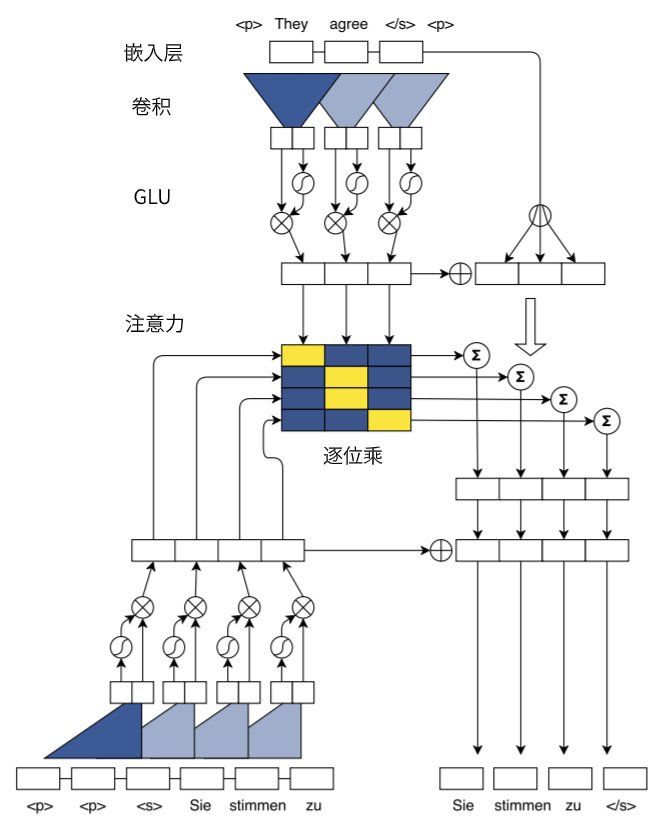
\includegraphics[width=0.8\textwidth]{figure/resources/CS2S_arch.png}
	\caption{\textbf{基于字卷积神经网络的后处理模块架构图}\label{CS2S_arch}}
\end{figure}

ConvS2S 的整体架构如图\ref{CS2S_arch}所示,其总体结构与 Transformer 类似的编码器解码器架构类似。
首先我们将输入 $\bm{x} = (x_1, \cdots, x_m)$ 词嵌入为 $\bm{w} = (w_1, \cdots, w_m)$,其中词嵌入维度为 $f$。
除了该词嵌入之外,额外引入了绝对值位置嵌入(可学习嵌入层):$\bm{p} = (p_1, \cdots, p_m)$,且维度与词嵌入相同。
我们只需要简单的把词嵌入与位置嵌入相加,便可以在序列中加入位置信息,即 $E = (x_1 + p_1, \cdots, x_m + p_m)$。
同样的,对于解码层的输入之一也就是已经解码的上文内容 $(y_1, \cdots, y_n)$,我们得到它的带位置信息的嵌入表示 $G = g_1, \cdots, g_n$。
解码器的目标就是得到当前解码内容 $p(y_{n+1}|y_1,\cdots,y_n, \bm{e})$。
不失一般性地,我们依然假设编码器和解码器都是 $L$ 层。

编码层和解码层中采用相同的卷积层区块,我们定义解码器的第 $l$ 层区块的输出为 $H_D^l \in \mathbb{R}^{n \times h}$,编码器的第 $l$ 层区块的输出为 $H_E^l \in \mathbb{R}^{m \times h}$。
对于输入为 $X \in \mathbb{R}^{k \times d}$,卷积核由参数 $W \in \mathbb{R}^{2d \times kd}, b_w \in \mathbb{R}^{2d}$构成,输出为 $Y = [A B] \in \mathbb{R}^{2d}$,激活单元为 GLU\cite{GLU}:

\begin{equation}
	\text{GLU}([A B]) = A \otimes \sigma(B)
\end{equation}
其中 $\sigma(\cdot)$ 为 sigmoid 函数,$\otimes$ 为逐位乘法。

为了使得网络更加深,我们在每一个区块之间加入残差连接。
为了保证序列长度在编码器不变,我们采用 \texttt{same padding}。
然而在解码层,我们要保证上文内容不包含任何下文,所以编码层上文输入首先在左右填充 $k-1$个零向量,然后在移除卷积输出的右边 $k$ 个输出。
对于解码器第 $l$ 层,卷积层输出为 $\hat{H}_D^l$,为了结合编码层最终输出的信息 $H_E^L$,我们使用多步注意力:

\begin{align}
	D^l &= \hat{H}_D^l W_d^l + b_d^l + G \\
	Z^L &= H_E^L W_z + b_z \\
	C^l &= \text{Attention}(D^l, H_E^L, H_E^L + E) \\
	H_D^l &= \hat{H}^L_D + C^l W_c
\end{align}
其中 $W_d, b_d, W_z, b_z$ 的目的是作为全连接层将 $H_D$ 和 $H_E$ 从 $h$ 维转换到 $f$ 维,$W_c \in \mathbb{R}^{f \times h}$。

最后编码层的当前编码结果就是 $p(y_{n+1}|y_1,\cdots,y_n, \bm{e}) = W^o H_{D,(n+1)}^L$。
其实也是类似与 Transformers,训练的时候因为上文就是完整输出延迟一个时间步的结果,的对于输出长度为 $m$ 的序列,输出是一次性完成,而在测试阶段只能一步一步解码。

\section{本章小结}

ConvS2S 模型的主要优点是在利用卷积运算获取的序列间以来的同时,使用 Attention 机制有机的讲编码器和解码器的内容结合了起来,同时还利用到了输入嵌入和上文嵌入的信息,并且还解决了编码器解码器输出序列长度不一致的问题。
随着 ConvS2S 在中文语法错误修正上的取得的成功,我们在本文寄希望于将 ConvS2S 网络作为 OCR 后处理模块对 OCR 识别内容的错误基于语义分析进行修正。

\chapter{基于语言模型的 Transformer 的 CRNN 语义修正后处理模块}
\label{chap:bert_nmt}

\section{方法概述}

本文跟随文献\cite{NLPCC}的思路,将 OCR 后处理作为一个特殊的由带有识别误差的文本到正确的文本的翻译任务。
鉴于 Transformer 在机器翻译领域取得的优越性能,我们决定使用 Transformer 作为我们的语义修正后处理模块的骨干结构。
此外,因为 OCR 识别结果中的错误往往在整段文本中只有少数几个错误。
这种带有个别错误的文本非常类似于 BERT 语言模型所使用的带掩码的语言模型任务,我们可以将识别错误视作一种特殊的掩码,并寄希望于它的上下文语义来为这些掩码提供一个预测。
并且,目前开源的大量 BERT 预训练模型为我们提供了丰富的资源,因为无监督学习的优势,这些预训练语言模型构建于超大规模语料库之上,这些语料库一般可以达到 100 亿汉字规模。
值得一提的是,如此规模的数据集,如果使用它们从头开始训练,这样的的资源消耗和训练时间对大多数研究者而言都是难以承受的,而预训练模型为我们节省了大量的资源占用和时间。
这样的规模一般远大于机器翻译所使用的源语言和目标语言句子对的数据及规模,在一定程度上可以弥补机器翻译或者本文所研究的语义修正任务使用的监督学习数据集在语言模型建模上的不足。
这样的思路主要来自于 BERT-NMT\cite{bert_nmt},该文献提出了一种融合 BERT 预训练模型和 Transformer 架构的模型,用于机器翻译,并在多个数据集上取得了新的最先进结果。
不同于 BERT-NMT,本文的针对 BERT-NMT 的改进如下:

\begin{enumerate}[(1)]
	\item 本文的目标任务为 OCR 识别结果的语义修正后处理模块,区别于机器翻译任务。
	\item 相对于 BERT-NMT 采用的原始版本 BERT 模型参数数量较大,基本上规模跟 Transformer 的编码器差不多。为了介绍资源消耗,同时利用 BERT 语言模型,我们采用 ALBERT\cite{albert} 模型作为语言模型。ALBERT 相对于 BERT 的特点是所有自注意力层共享相同的参数,这样极大的减少了显存占用,并且模型性能于 BERT 类似。
	\item 因为本文主要针对中文 OCR 识别结果,并且结果中含有识别错误。所以不同于 BERT-NMT 等机器翻译模型会将输入首先分词或切分成更小的单元以获得性能提示并缓解超出词典范围的情况,我们不采用任何分词手段,模型的输入以字为单位。
\end{enumerate}

接下来的小节中,我们将首先在第\ref{notation}小节中,我们将首先介绍符号约定,以及整个模型的总体流程图,以便读者对我们提出的模型树立一个初步且全面的认识。
随后,在第\ref{postprocess}小节,基于 ALBERT 和 Transformner 的 OCR 语义修正后处理模块的详细结构和形式化描述将在该小节中展开。
最后,在小节\ref{conclusion_bert_ocr}中,我们总结我们的模型,并讨论其与相关研究的优劣之处。

\section{符号约定及流程图}
\label{notation}
首先定义按照文本行语义分割后的灰度图为 $\bm{m} \in \mathbb{R}^{h \times w}$,高度为 $h$,宽度为 $w$。
字典为 $\mathcal{V}$,则 CRNN 的输出结果为:

\begin{equation}
	\bm{h} = \text{CRNN}(\bm{m})
\end{equation}
其中 $\bm{h} \in \mathbb{R}^{(w / 4 - 1) \times |\mathcal{V}|}$。

也就是说,CRNN 的输出为 $w / 4 - 1$ 个字符,其中每一个行向量为它在字典上的概率分布。
这里我们采用简单的基于贪心算法的解码器,我们取每个行向量中最大概率所对应的字符为该位置的识别字符。
随后,我们使用 CTC 解码函数 $\mathcal{B}$,得到最终的 CRNN 文本识别结果:

\begin{equation}
	\bm{x} = \mathcal{B}([\arg \max(\bm{h}_i)]_i)
\end{equation}
其中识别结果 $\bm{x} \in \mathbb{R}^{l_x}$ 是一个长度为 $l_x$ 的文本的数值化后的序列。

该是被结果 $\bm{x}$ 中可能存在识别误差,接着我们定义对应的正确结果 $\bm{y} \in \mathbb{R}^{l_y}$ 为长度为 $l_y$ 的序列。
因为可能存在多种错误,所以有可能 $l_y \ne l_x$。
我们将 ALBERT 模型作为一个单独的模块 \texttt{BERT}。
类似 Transformer 的编码器-解码器结构,不过不失一般性地,我们假定编码层和解码层的层数均为 $L$。
自注意力层和逐位前馈层,同样类似 Transformer,并且我们定义他们为 $\texttt{attn}(Q, K, V)$ 和 $\texttt{FFN}(h)$。

\begin{figure}[h!]
	\centering
	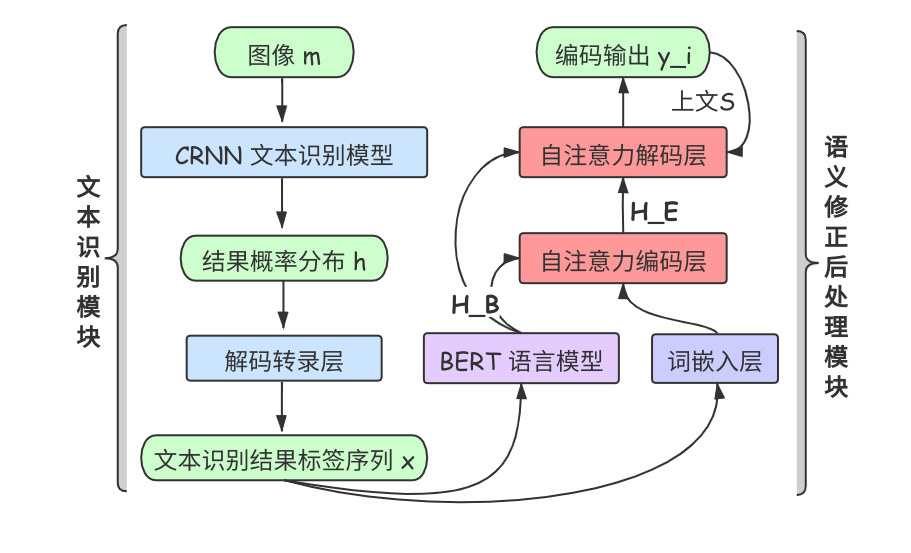
\includegraphics[width=0.8\textwidth]{figure/resources/overall.png}
	\caption{\textbf{CRNN 文本识别及基于语言模型的 Transformer 的后处理模块流程图}\label{overall_arch}}
\end{figure}

完整的流程图在图\ref{overall_arch}中展示。
本文实现的文本识别系统主要分为两个模块:(1) CRNN 文本识别模块,(2) 基于 ALBERT 语言模型的 Transformer 后处理模块。
首先 CRNN 文本识别模块已经在第\ref{crnn}小节中较为详细的描述,在我们输入图片 $\bm{m}$ 后,CRNN 的输出经过解码转录后得到标签序列 $\bm{x}$。
随后,我们将带有识别误差的 $\bm{x}$ 输入到基于 ALBERT 语言模型的 Transformer 后处理模块中。
该后处理模块在 Transformer 的编码器-解码器结构之外额外新增了 ALBERT 语言模型的输出结果,用于对编码器和解码器进行强化。
对于编码器,编码器的输入为 $\bm{x}$ 的词嵌入表示和 ALBERT 语言模型的输出。
在解码过程中,解码器的输入为 ALBERT 语言模型输出,最后一层自注意力编码器的输出,以及之前编码的内容作为上文信息。
注意对于 ALBERT 预训练模型,其字典与我们的系统使用的字典不一致,所以在这里我们需要首先使用我们的字典将标签序列 $\bm{x}$ 转化为文本,随后使用 ALBERT 预训练的字典和令牌解析器(tokenizer)进行数值化。
因为空间问题我们在流程图中没有标明这一转换过程。
对于预训练 ALBERT,我们使用 \texttt{albert\_zh}\footnote{albert\_zh: \url{https://github.com/brightmart/albert_zh}} 提供的预训练模型。
然后使用 huggingface 开发的框架\footnote{huggingface transformers: \url{https://github.com/huggingface/transformers}}方便地加载和使用这些预训练模型。

\section{语义修正后处理模块}
\label{postprocess}

本小节我们主要详细介绍语义修正后处理模块的结构和公式。
该后处理模块的架构在图\ref{postprocess_arch}中展示,虚线表示残差连接\cite{ResNet},当起点连接至层范化层时,表示残差连接的输入为该层范化层的输出,而如果虚线的终点连接至层范化层时,表示残差连接的输出作为该层范化层的输入。
不同于 Transformer 的三种自注意力层,我们的语言修正模块额外使用一种新的自注意力层:ALBERT 自注意力层。
该 ALBERT 自注意力层负责将 ALBERT 的输出作为值和键,而将编码层或者解码层的输入作为查询,进而将 ALBERT 对 $\bm{x}$ 的语言模型表示与编码器和解码器所学到的中间表示进行融合,充分利用这二者学习的特征。


\begin{figure}[h!]
	\centering
	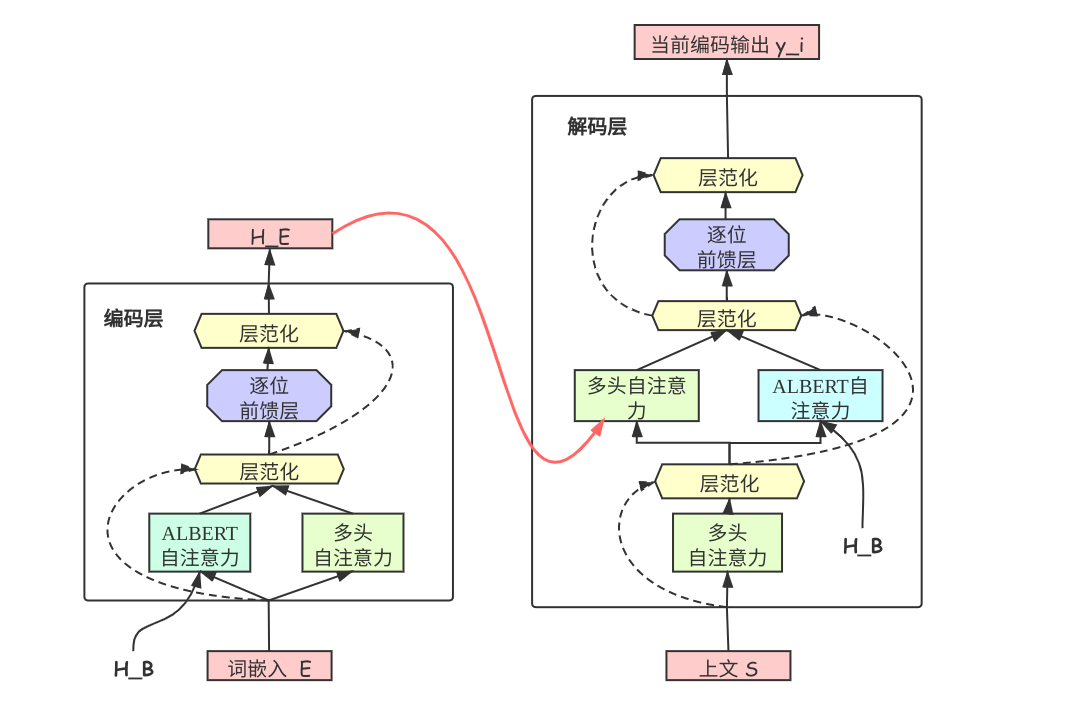
\includegraphics[width=0.95\textwidth]{figure/resources/ALBERT_NMT.png}
	\caption{\textbf{语义修正后处理模块架构图}\label{postprocess_arch}}
\end{figure}


首先我们定义 ALBERT 语言模型的最后一层输出为 $H_B = \texttt{BERT}(\bm{x}), H_B\in \mathbb{R}^{l_x \times h_b}$。
对于编码器的第 $l$ 层隐藏表示输出,定义为 $H_E^l$,其中 $H_E^0$ 表示第一层编码层的输入,也就是 $\bm{x}$ 经过嵌入层的词嵌入表示。
对于其中$H_E^l$的第 $i$ 个位置我们表示为 $h_i^l, i \in [l_x]$,所以对于第$l$层编码层,我们有:

\begin{equation}
	\label{encoder}
	\hat{h}_i^l = \frac{1}{2} (\texttt{attn}_S(h^{l-1}_i, H_E^{l-1}, H_E^{l-1}) + \texttt{attn}_B(h_i^{l-1}, H_B, H_B)), \forall i \in [l_x]
\end{equation}
其中 $\texttt{attn}_S, \texttt{attn}_B$ 表示具有不同参数的自注意力模块。
所以经过逐位前馈层后,对于第 $l$ 层隐藏表示输出为:

\begin{equation}
	H_E^l = (\texttt{FFN}(\hat{h}_1^l), \cdots, \texttt{FFN}(\hat{h}_{l_x}^l))
\end{equation}

接着,我们定义在时间步 $t$ 时,此时解码层的输入我们定义为 $S_{<t}^l = (s_1^l, \cdots, s_{t-1}^l)$。
其中对于第一层解码层,$s_t^0$ 为已经解码的上文的第 $t$ 个词嵌入。
所以,第 $l$ 层解码层的隐藏表示我们定义为:

\begin{equation}
	\label{decoder}
	\hat{s}_{t}^l = \texttt{attn}_S(s_t^{l-1}, S_{<t}^{l-1}, , S_{<t}^{l-1}) \\
	\hat{s}_{t}^l = \frac{1}{2}(\texttt{attn}_B(\hat{s}_t^{l}, H_B, H_B) + \texttt{attn}_E(\hat{s}_t^l, H_E^l, H_E^l)) \\
	s_t^l = \texttt{FFN}(\hat{s}_t^l)
\end{equation}
其中 $\texttt{attn}_S, \texttt{attn}_B, \texttt{attn}_E$ 分别表示三种不同参数的自注意力层。
公式\ref{decoder}在解码过程中会被重复执行,维度为 $d_m$ 的隐藏表示最终经过线性变换层和 softmax 激活单元后每次输出一个字符,直至输出特殊标识符 \texttt{[EOS]} 后停止。
代表此时已经解码完成,解码出了完整的经过后处理模块语义修正后的文本。

在本方法中,因为我们同时使用了两种类型的 Transformer 架构,这会导致我们的模型较为复杂,也就是说表示空间会比较大。
为了避免增加 ALBERT 所带来的过拟合风险,我们参考 dropout\cite{dropout} 以及 BERT-NMT\cite{bert_nmt} 所提出来的 dropnet 技术来作为正则化手段。
首先我们定义 drop-net 的概率为 $p_{\text{drop}} \in [0,1]$。
类似与 dropout,在训练的时候,对于网络中的每一层 $l$,我们首先从均匀分布采样一个值 $U^l \sim \text{Uniform}(0,1)$,然后对于编码层,公式\ref{encoder}将变为:

\begin{align}
	\label{encoder_drop}
	\hat{h}_{i,\text{drop-net}}^l &= \mathbb{I}(U^l < \frac{p_{\text{drop}}}{2}) \cdot \texttt{attn}_S(h^{l-1}_i, H_E^{l-1}, H_E^{l-1}) + \mathbb{I}(U^l > 1 - \frac{p_{\text{drop}}}{2} \cdot \texttt{attn}_B(h_i^{l-1}, H_B, H_B)) \nonumber \\
	&+ \frac{1}{2} \mathbb{I}(\frac{p_{\text{drop}}}{2} \le U^l \le 1 - \frac{p_{\text{drop}}}{2}) (\texttt{attn}_S(h^{l-1}_i, H_E^{l-1}, H_E^{l-1}) + \texttt{attn}_B(h_i^{l-1}, H_B, H_B))
\end{align}
其中 $\mathbb{I}$ 表示表示标志函数,即如果其中参数为真则返回 1 否则返回 0。
这样做的目的是,在某一层,有一定概率只使用 ALBERT 自注意力 $\texttt{attn}_B$,也有一定概率只使用自注意力层 $\texttt{attn}_S$,也有一定概率两者同时使用。

同样的,在训练过程中,对于解码层的隐藏表示,我们也有:

\begin{align}
	\label{decoder_drop}
	\hat{s}^l_{t,\text{drop-net}} &=\mathbb{I}(U^l < \frac{p_{\text{drop}}}{2}) \cdot \texttt{attn}_S(\hat{s}_t^{l}, H_E^{l-1}, H_E^{l-1}) + \mathbb{I}(U^l > 1 - \frac{p_{\text{drop}}}{2} \cdot \texttt{attn}_B(\hat{s}_t^{l}, H_B, H_B)) \nonumber \\
	&+ \frac{1}{2} \mathbb{I}(\frac{p_{\text{drop}}}{2} \le U^l \le 1 - \frac{p_{\text{drop}}}{2}) (\texttt{attn}_S(\hat{s}_t^{l}, H_E^{L}, H_E^{L}) + \texttt{attn}_B(\hat{s}_t^{l}, H_B, H_B))
\end{align}

类似于 dropout,我们同样需要在测试时修正 dropnet。
因为公式\ref{encoder_drop}的数学期望就是公式\ref{encoder},而公式\ref{decoder_drop}的数学期望也同理就是公式\ref{decoder}。
所以在测试阶段,我们只需要简单的把公式\ref{encoder_drop}和公式\ref{decoder_drop}换回公式\ref{encoder}和公式\ref{decoder}即可。

\section{本章小结}
\label{conclusion_bert_ocr}
本章节首先介绍了我们提出的面向语义分析的文本识别系统的整体流程图。
随后我们介绍了在后处理模块中使用 ALBERT 预训练语言模型的动机和优势。
在最后我们详细介绍基于 ALBERT 语言模型和 Transformer 的 OCR 语义修正后处理模块,并用数据公式和架构图相辅对该后处理模块进行了详细的介绍。
并且,为了解决过拟合问题,我们提出使用一种 dropout 的变种用于正则化手段。
总得来说,我们提出的后处理模块类似于翻译任务,把 OCR 识别出来的可能带有识别误差的结果当作源语言,而将正确的结果当作目标语言。
修正的过程即是一个翻译的过程。
同时,因为带有识别误差的结果类似 BERT\cite{bert} 等语言模型所采用的带掩码的语言模型,所以基于这个发现,我们提出使用 ALBERT\cite{albert} 语言模型辅助增强我们的后处理模块对 OCR 识别结果的语言模型的感知与特征提取。
除了我们的模型所带来的好处之外,因为 ALBERT 模型的引入,我们的后处理模块不可避免的需要产生较多的额外消耗,同时 Transformer 相对于卷积神经网络来说,其庞大的参数数量确实需要更加大的资源消耗。
不过相对于 BERT-NMT\cite{bert_nmt},ALBERT 的使用减少了语言模型所带来的资源占有。

\chapter{实验步骤}
\label{chap:experiments}
本章节将我们详细介绍我们的实验步骤,并且将测试多种方法作为后处理模块以及原始不带后处理模块的 CRNN 模型。
此外,我们还将探究 ALBERT 的使用是否带来帮助,以及 dropnet 对模型性能的影响。
首先我们将在第\ref{exp_env}小节展示我们的实验软硬件环境,在\ref{dataset}小节中介绍我们采用的数据及以及数据增强技术,随后,我们在第\ref{exp_design} 介绍我们的实验设计以及评价指标。
实验结果和分析将在第\ref{result}小节展示和讨论,最后在第\ref{exp_conclusion}小节中我们总结本章节的内容。

\section{实验软硬件环境}
\label{exp_env}
本文的实验主要基于一台三卡 GPU 服务器,其具体硬件配置信息如表\ref{tab:conf}所示。

\begin{table}[!hpt]
	\caption[]{\textbf{GPU 服务器硬件配置}}
	\label{tab:conf}
	\centering
	\begin{tabular}{c c}
		\hline
		\textbf{属性名} & \textbf{属性值} \\ [0.5ex] 
		\hline
		CPU1 & Intel(R) Xeon(R) Silver 4210 (10核20线程) \\
		CPU2 & Intel(R) Xeon(R) Silver 4210 (10核20线程) \\
		GPU1 & NVIDIA GeForce GTX 2080Ti(12G显存) \\
		GPU2 & NVIDIA GeForce GTX 2080Ti(12G显存 \\
		GPU3 & NVIDIA GeForce GTX 2080Ti(12G显存)\\
		内存 & 128GB \\
		磁盘容量 & 4TB \\
		\hline
	\end{tabular}
\end{table}

值得一提的是,GTX 2080Ti 支持半精度(FP16)训练,这可以降低神经网络的显存占用,并且加快计算速度。
所以后续实验中,对于能够开启 FP16 的情况,我们均开启了半精度。

本文的实验代码主要基于 Facebook 开源的 Fairseq\cite{ott2019fairseq} 序列到序列工具库,Fairseq 实现了多种翻译模型:包括但不限于注意力机制 LSTM\cite{attn_lstm},字卷积神经网络\cite{cs2s},以及 Transformer\cite{transformer}。
对于 ALBERT 预训练模型,我们使用 albert\_zh 提供的预训练模型,名称为 \texttt{albert\_tiny\_google\_zh}。
相比于 BERT,\texttt{albert\_tiny\_google\_zh} 层数仅为4层、隐藏表示等向量维度大幅减少,训练和推理预测速度提升约10倍,精度基本保留,模型大小为 BERT 的1/25。
其训练数据为30G中文语料,超过100亿汉字,包括多个百科、新闻、互动社区。
预训练序列长度设置为512,批次大小为4096,训练产生了3.5亿个训练数据,训练$12.5$万步。

对于 CRNN 模型,我们的实现主要基于 cnocr \footnote{cncor: \url{https://github.com/breezedeus/cnocr/}} 项目。
对于基于 ALBERT 和 Transformer 的语义修正后处理模块,我们主要参考并修改了 BERT-NMT\footnote{BERT-NMT: \url{https://github.com/bert-nmt/bert-nmt}} 提供的代码。


\section{数据集与数据增强}
\label{dataset}
鉴于大多数开源中文文本识别数据集对于我们的语义修正后处理模块存在以下几个问题:

\begin{enumerate}[(1)]
	\item 场景文本识别任务的数据主要来源与街景照片,例如广告牌、交通标识、商店招牌等,这些内容往往存在文本行较短(例如两三个字)或者没有明显语义信息(例如商店名称)。这样的数据集包括 ICDAR RCTW-17\cite{RCTW}和 ICDAR 2019 LSVT\cite{lsvt}。
	\item 类似于翻译任务,我们后处理模块需要大量的句子对数据,也就是带有 OCR 识别误差的样本和对应的正确的样本。因为数据规模的要求,大多数公开数据集,规模一般在几千到数十万,不能很好的满足我们的训练需求。
\end{enumerate}

因此,我们决定自己创造数据集,我们选择采用人工合成数据集,因为这样能够快速创建大量的带标注的数据。
首先对于语料库,我们选择使用开源中文文本数据及 THUCNews。
THCNews 数据集来源于 THUCTC\cite{sum2016thuctc} 项目,该数据集来源于新浪新闻RSS订阅频道在 $2005~2011$年的新闻文章,大小为 (2.19 GB),采用 UTF-8 编码。
该数据及总共包含74万篇新闻文。
不同于新浪新闻的分类体系,THUCNews 将数据集划分成14种类,并且每个类的样本是不平衡的。
因为我们需要从文本中生成图像,如此规模的数据如果全部用作生成我们的数据集,产生的图片大小是难以承受的。
所以我们对于每个类均匀随机采样 $30000$ 行文本。

\begin{figure}[h!]
	\centering
	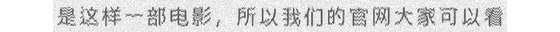
\includegraphics[width=0.8\textwidth]{figure/resources/sample.png}
	\caption{\textbf{数据集中的样本实例}\label{sample}}
\end{figure}

因为训练 CRNN 的时候,文献\cite{CRNN} 推荐所有样本固定长度。
所以我们对所有文本行分割为长度为 $18 \sim 20$ 字符的文本。
最终我们生成的文本行数量为 $1637012$,其中字典大小为 $6425$。
该字典涵盖所有英文字符,常见中英文标点符号,以及常见中文字符。
接着,对于每一个文本行,我们使用开源项目 TextRecognitionDataGenerator\footnote{TextRecognitionDataGenerator: \url{https://github.com/Belval/TextRecognitionDataGenerator}},生成对应的图像作为一个最终数据样本。
TextRecognitionDataGenerator 支持选择不同的字体,以及制定不同的数据增强技术,以增加数据的复杂度。
具体来说,我们收集了 70 中不同的中文字体,对于 THUCNews 的每一个类,我们均匀的选用不同的字体。
文本的颜色范围为 $\#000000 \sim \#888888$。
文本畸变(distorsion)我们采用随机算法,图片背景采用高斯噪声。
最终生成的图像为大小固定为 $(32, 560)$ 的 RGB 彩色照片,不足该大小的,我们会首先缩放其高度至 32, 然后用纯白色背景在图像左右均匀填充以达到 560 的长度,字符之间的间隙为 6 个像素。
对于这些生成的 RGB 彩色图像,为了减小存储空间,并且遵循 CRNN\cite{CRNN} 的设置,我们首先会使用 PIL 库将其转换为灰度图,然后存储到 hdf5 文件。
最终数据集的样本,如图\ref{sample}所示,它对应的标签是“是这样一部电影,所以我们的官网大家可以看”。

\section{实验设计}
\label{exp_design}
首先我们将数据集按照 $8:2$ 的比例分为训练集和测试集,其中测试集大小为 $327403$,训练集大小为 $1309609$。
我们首先使用训练集合中所有的图片作为数据集,对预训练的 CRNN 进行微调训练。
微调训练采用两块 2080Ti 显卡,优化器使用 Adam,学习率度固定为 $10^{-3}$,额外训练三代。
因为预训练模型采用 cnocr 提供的代码,其数据集与我们创建的 hdf5 数据集的加载方式不一致。
所以我们额外创建了一个数据集加载器类,批次大小为 $128$,drpout 率为 $0.5$。
在训练过程中,我们为了增加模型的鲁棒性,我们额外增加了一些数据增强技术:

\begin{enumerate}[(1)]
	\item 亮度抖动范围为 $0.001$
	\item 对比度抖动范围为 $0.001$
	\item 饱和度抖动范围为 $0.001$
	\item 色相抖动范围为 $0.05$
	\item PCA 噪声等级为 $0.1$
	\item 采用基于面积的插值算法
	\item 前景色背景色随机对调概率为 $0.2$
\end{enumerate}

接着,我们使用微调后的 CRNN 模型推理包括训练集和测试集的所有样本以便得到足够多的带有 OCR 识别错误的结果。
注意,为了进一步增加数据多样性,我们在 CRNN 的转录层随机采用两种不同的解码算法:

\begin{enumerate}[(1)]
	\item \textbf{基于贪心算法的 CTC 解码器}:对于每一个时间步的概率分布,我们简单的选择概率最大的标签作为预测标签,然后使用 CTC 解码函数 $\mathcal{B}$ 消除重复字符和空字符。
	\item \textbf{基于束搜索的 CTC 解码器}\cite{ctc_beam}:在每个时间步会保留 $n$ 个结果,并且按照 CTC 算法计算概率的特点,最后找到评分最高的路径对应的结果作为预测结果。值得一提的是,在打分过程中,可以使用额外的 $n$-gram 打分器。因为我们实验发现 $n$-gram 外部打分器用处不大,而且我们的目的是得到足够多的带有 OCR 识别错误的样本,所以我们没有采用 $n$-gram 打分器。
\end{enumerate}

最后我们得到的 CRNN 识别结果中,在训练数据集(大小为 $1309609$)上,我们微调的 CRNN 能够正确识别整个句子的有 $843522$ 个样本,精确率为 $0.6441$。
在大小为 $327403$ 的测试集上,微调的 CRNN 能够正确识别整个句子的有 $210426$ 个样本,精确率为 $0.6427$。

最后我们得到的用于语义修正后处理模块的数据集中每一个样本为带有识别错误的结果和正确的结果的句子对。
例如 CRNN 对某一训练集样本的识别结果为 “\textbf{\textcolor{red}{罩}注\textcolor{red}{樊}金按注均分,\textcolor{red}{!}注最高限额封顶500}”,而正确结果为 “\textbf{单注奖金按注均分,单注最高限额封顶500}”,该识别结果共有三个替换错误。
因为得到的训练集样本中约 $2/3$ 为没有任何识别错误的结果,相比于带识别错误的结果比例不平衡,所以我们对训练集中识别完全正确的样本采用下采样技术,也就是随机丢弃 $50\%$ 的识别完全正确的结果。

对于测试阶段的评价函数,我们主要使用两种。
一种是完整匹配(EM)精确度,其公式可以定义为:

\begin{equation}
	\text{EM 精确度} = \frac{\text{后处理模块预测结果与正确结果完整匹配的数量}}{\text{总样本数}}
\end{equation}

另一种我们称为 Levenshtein 编辑距离\cite{levenshtein1966binary}归一化分数.
Levenshtein 编辑距离为从源句子到目标句子说需要的编辑操作数,编辑操作共三种:替换(replace)、删除(delete)插入(insert)。
例如对于 OCR 识别结果和正确结果句子对 \texttt{[',还你无明白棘肌肤', '还你无暇白嫩肌肤!']},总共需要 4 个编辑操作为 \texttt{[('delete', 0, 0), ('replace', 3, 3), ('replace', 5, 5), ('insert', 9, 9)]}。
我们定义其公式为:

\begin{equation}
	\text{Levenshtein 分数} = 100 \times (1 - \frac{\text{后处理模块预测结果与正确结果的 Levenshtein 编辑距离}}{\text{后处理模块预测结果与正确结果中的最大长度}})
\end{equation}

\section{实验结果与分析}
\label{result}

除了不经过语义后处理模块的 CRNN 直接识别结果外,我们实现了三种基于语义的后处理模块:

\begin{enumerate}[(1)]
	\item 基于字卷积神经网络的,以下简称 \textbf{ConvS2S 模型}。
	\item 基于 Transformer 的,以下简称 \textbf{Transformer 模型}。
	\item 基于 ALBERT 预训练语言模型和 Transformer的,以下简称 \textbf{ALBERT-Transformer 模型}。
\end{enumerate}

\begin{figure}[h!]
	\centering
	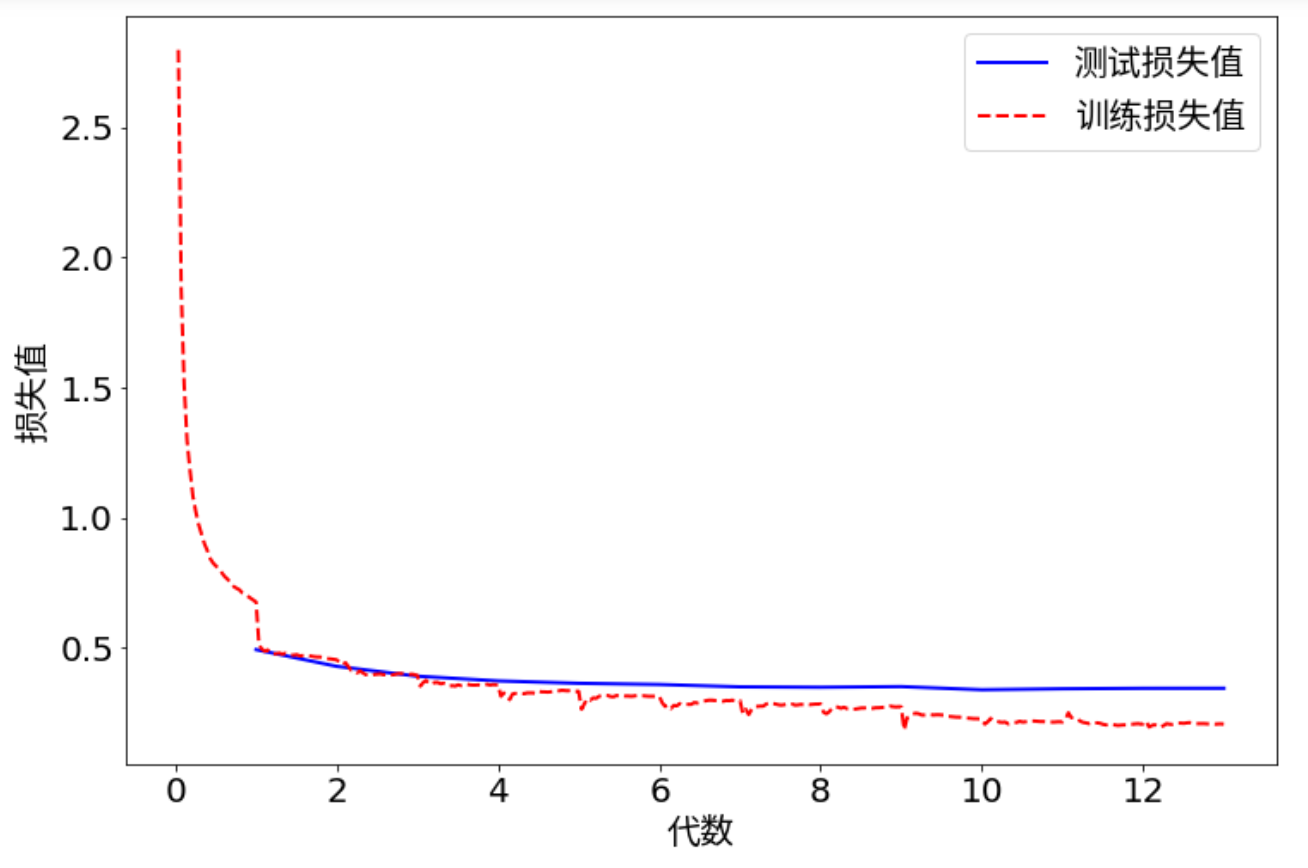
\includegraphics[width=0.8\textwidth]{figure/resources/loss_cs2s.png}
	\caption{\textbf{ConvS2S 的训练曲线}\label{loss_cs2s}}
\end{figure}

\begin{figure}[h!]
	\centering
	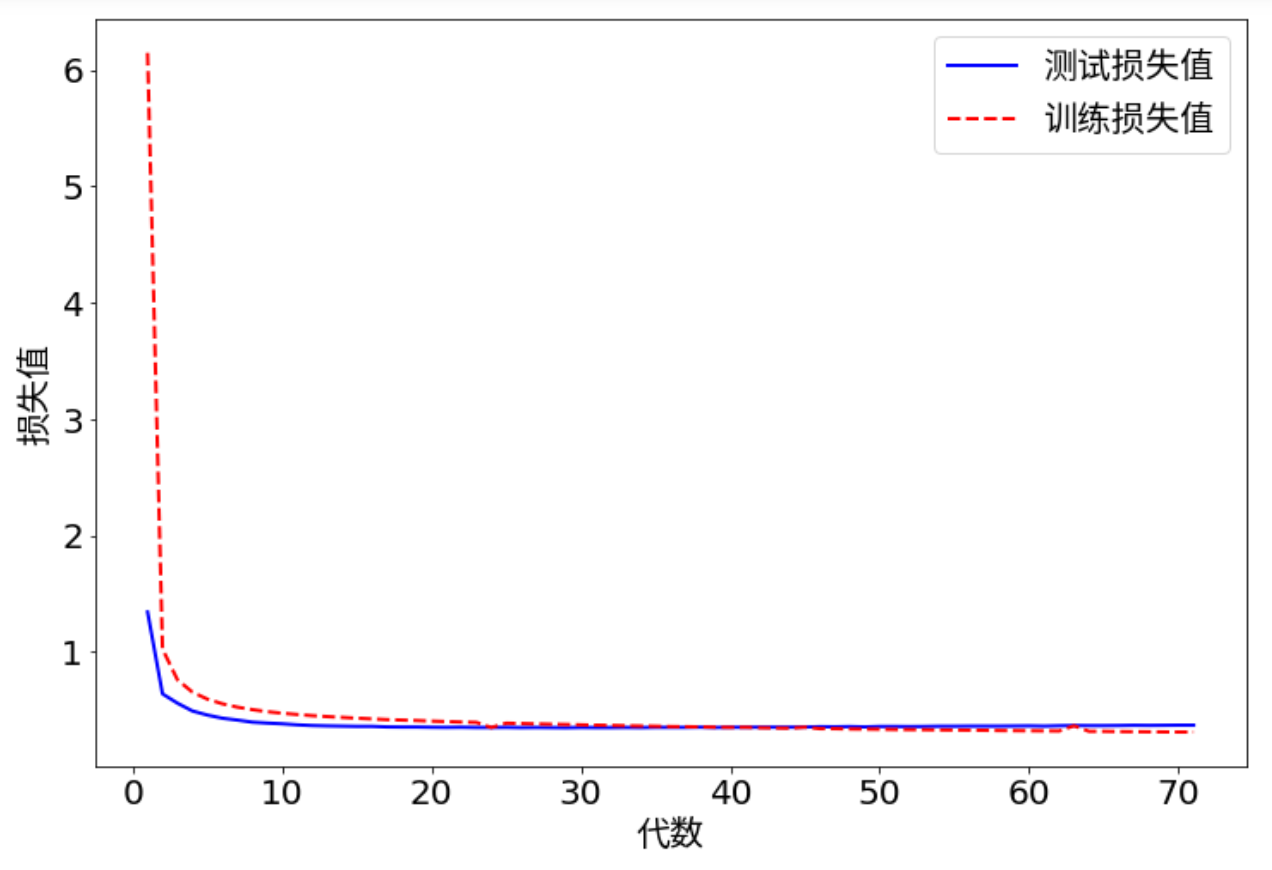
\includegraphics[width=0.8\textwidth]{figure/resources/loss_transformer.png}
	\caption{\textbf{Transformer 的训练曲线}\label{loss_transformer}}
\end{figure}

首先我们介绍这些模型的参数。
ConvS2S 的批次大小为 32,损失函数为交叉熵,dropout 率为 $0.2$,编码层和解码层均为 7 层,隐藏特征的输出维度为 $1024$,卷积核大小为 3。
初始学习率为 $0.25$,学习率调度器采用 \texttt{reduce\_lr\_on\_plateau},也就是说,如果损失值连续多代不再降低时,会将当前学习率缩放 $0.1$
输入、输出和上文的嵌入层维度均为 500。
总参数规模为 $106,449,810$。

Transformer 的超参数主要有:Adam 优化器参数为 $(0.9, 0.98)$,编码器和解码器的自注意力头均为 $4$,自注意力的隐藏表示维度为 $512$,逐位前馈层的维度为 $1024$,编码器和解码器的层数为 6,dropout 率为 $0.3$,权重惩罚项系数 $0.0001$,初始化学习率为 $0.0005$,学习率调度器采用先缓慢上升在按照平方根的倒数来下降,标签平滑交叉熵系数为 $0.1$,采用半精度浮点数训练,批次大小为 $256$。
总参数规模为 $37,220,352$。

ALBERT-Transformer 因为总体结果类似 Transformer,所以除了与上述 Transformer 的参数一致,额外的超参数有:dropnet 率为 $0.4$,并且不重新进行训练,直接用上述 Transformer 的预训练模型中进行微调。
微调的批次大小为 512,初始热启动学习率为 $10^{-7}$,最小学习率为 $10^{-9}$。

对于对比方法,本文选择使用第\ref{n_gram}节中介绍的基于 $n$-gram 和迷惑集的方法,$n$-gram 我们使用 KenLM 工具在我们创建的数据集上构建 $3$-gram 语言模型,迷惑集我们采用数据集中编辑操作为替换的字符,完整的修正框架我们使用开源的 \texttt{pycorrector}\footnote{pycorrector: \url{https://github.com/shibing624/pycorrector}}。

\begin{table}[!hpt]
	\caption[]{\textbf{drop-net 率参数调整实验结果}}
	\label{tab:result_dropnet}
	\centering
	\begin{tabular}{c c c}
		\hline
		\textbf{drop-net 率} & \textbf{EM 精确度} & \textbf{Levenshtein 分数} \\
		\hline
		0.0 & 0.8320 & 94.3315 \\
		0.1 & 0.8347 & 94.2958 \\
		0.4 & \textbf{0.8483} & \textbf{94.3760} \\
		1.0 & 0.8453 & 94.3633 \\
		\hline
	\end{tabular}
\end{table}

对于 ALBERT-Transofmer,BERT-NMT\cite{bert_nmt} 推荐 drop-net 率为 $1.0$,也就是训练时某一层要么只有 ALBERT 自注意力,要么只有 Transformer 自注意力。
我们发现该值在我们的 OCR 识别结果后处理模块中效果并不好,于是我们通过实验对这个参数进行调整。
具体的实验结果在表\ref{tab:result_dropnet}中展示。
通过是实验结果,我们发现 $0.4$ 是比较适合我们的应用场景的值。

\begin{table}[!hpt]
	\caption[]{\textbf{对比实验结果}}
	\label{tab:result}
	\centering
	\begin{tabular}{c c c}
		\hline
		\textbf{方法名称} & \textbf{EM 精确度} & \textbf{Levenshtein 分数} \\
		\hline
		CRNN & 0.6420 & 94.0595 \\
		CRNN + $n$-gram & 0.6427 & 94.0927 \\
		CRNN + ConvS2S & 0.8461 & 94.3130 \\
		CRNN + Transformer & 0.8421 & 94.2802 \\
		CRNN + ALBERT-Transformer & \textbf{0.8483} & \textbf{94.3760} \\
		\hline
	\end{tabular}
\end{table}

ConvS2S 和 Transformer 的训练曲线如图\ref{loss_cs2s}和图\ref{loss_transformer}所示,因为 ALBERT-Transformer 的训练曲线类似于 Transformer,我们就不展示 ALBERT-Transformer 的训练曲线了。
从图中可以看出,虽然本实验中的 ConvS2S 模型的参数规模更加大,但是 ConvS2S 训练收敛速度很快,在第 4 代时已经明显收敛,并且在随后出现了第八代开始出现过拟合现场。
另一方面,Transformer 在第 10 代才开始收敛,并且一直到第 70 代,也没有出现过拟合现场。
我们认为这是因为 ConvS2S 的初始学习率很高($0.25$),而 Transformer 的初试学习率很低($0.0005$)。
并且 Transformer 学习率调度器会缓慢增加在缓慢降低,而 ConvS2S 的学习率调度器为如果损失值不降低就直接将学习率降低 $90\%$。
所以我们可以在训练曲线中看出,ConvS2S 的训练曲线有波动,这是因为学习率调度器发现损失值不再降低后调整学习率后导致的,而 Transformer 的训练曲线及其平缓。

在训练收敛后,我们将我们训练的三中神经网络作为 OCR 语义修正后处理模块进行测试,并且评价指标我们选择使用完整匹配精确度和编辑距离归一化分数。
对于原始的没有经过后处理模块修正的 CRNN 识别结果,详细的实验结果在表\ref{tab:result}中展示,得分最高的项目由粗体标明。
从表中可以看出,这四种后处理模型的性能分别是 $\text{ALBERT-Transformer} > \text{ConvS2S} > \text{Transformer} > \text{n-gram}$。
并且即使是分数较低的 Transformer,其 EM 精确度提高了 $0.2001$,提升效果明显。
而对比方法——基于 $n$-gram 的后处理模块表现较差,提升很少,这是因为 $n$-gram 语言模型的能力有限,并且迷惑集依赖专家经验,我们提供的迷惑集只是简单的对数据集中的替换错误收集了起来。
同时,我们可以发现,虽然 EM 精确度提升明显,但是 Levenshtein 编辑距离分数提高百分比并不是更高。
这是因为,我们的数据集中,或者说在一般的 OCR 应用场景中,大部分识别错误都只是一两个字的错误,所以对编辑距离的影响不是很大。
而数据集中仍然有一些(一万左右)整句话基本全部识别错误的样本,对于这样的错误,后处理模块因为无法得到足够的语义信息,所以基本很难对这样的识别错误进行修正。

\begin{table}[!hpt]
	\caption[]{\textbf{基于语义分析的后处理修正模块成功案例}}
	\label{tab:success}
	\centering
	\begin{tabular}{c c}
		\hline
		\textbf{OCR 识别结果} & 英格兰银行的通货膨\textbf{服}目\textbf{模}为2\%。根据国 \\
		\textbf{识别错误类型} & 替换+插入 \\
		\textbf{语义修正结果} & 英格兰银行的通货膨\textbf{胀}目\textbf{标}为2\%。根据国\textbf{际} \\
		\hline
		& \\
		\hline
		\textbf{OCR 识别结果} & 仍由民政部与\textbf{罔}家\textbf{休}体育\textbf{鹅}局具休制定和\textbf{宵}施。 \\
		\textbf{识别错误类型} & 删除+替换 \\
		\textbf{语义修正结果} & 仍由民政部与\textbf{国}家体育总局具体制定和实施 \\
		\hline
	\end{tabular}
\end{table}

\begin{table}[!hpt]
	\caption[]{\textbf{基于语义分析的后处理修正模块失败案例}}
	\label{tab:fail}
	\centering
	\begin{tabular}{c c}
		\hline
		\textbf{OCR 识别结果} & 活家禽批发商会预计,零\textbf{傅}价约为每斤2\textbf{G}6元 \\
		\textbf{语义修正结果(ALBERT-Transformer)} & 活家禽批发商会预计,零售价约为每斤66元 \\
		\textbf{语义修正结果(ConvS2S)} & 活家禽批发商会预计,零售约为每斤2G6元 \\
		\textbf{实际正确结果} & 活家禽批发商会预计,零售价约为每斤26元 \\
		\hline
		& \\
		\hline
		\textbf{OCR 识别结果} & “我\textbf{冈图}密室部分,\textbf{区}(指\textbf{因}佩慈)\textbf{因因}不可 \\
		\textbf{语义修正结果(ALBERT-Transformer)} & “我们紧密室部分,谢(指导佩慈)发现不可 \\
		\textbf{语义修正结果(ConvS2S)} & “我们亲密室部分,谢(指纹佩慈)因为不可 \\
		\textbf{实际正确结果} & “我负责密室部分,她(指吴佩慈)负责不可 \\
		\hline
	\end{tabular}
\end{table}

我们在表\ref{tab:success}中展示了一些典型的被我们的后处理模块成功修正的 OCR 识别错误案例,OCR 识别结果中错误的地方和对应的修正结果用粗体标识。
我们可以看到对于 OCR 识别结果中的错误,如果错误是个别字符,模型可以基于上下文将其修正,包括替换、删除和插入。
这样的成功案例在词组中部分字别识别错误时比较常见,例如像表中第二个例子“\textbf{体育总体}”这种固定词组,我们提出的后处理模块很容易将“\textbf{体育鹅局}”中的错误发现并识别,
同时在表\ref{tab:fail}中我们也展示了一些没有被成功修正的案例。
总的来说,我们发现这些后处理模块识别结果中的个别替换错误,如果上下文仍然比较清楚的时候,比较容易发现和修正,如果因为识别错误过多,上下文不清楚的时候,很难成功修正。
并且,我们发现我们提出的后处理模块更加擅长替换错误,而对于插入错误和删除错误的成功率就比较低了。

\section{本章小结}
\label{exp_conclusion}

本章节系统全面的介绍了本文实验的软硬件环境以及实验设计和结果分析。
对 ALBERT-Transformer,本章还实验讨论了其超参数 drop-net 的取值。
从实验结果上看,文本提出的后处理模块对 CRNN 的识别结果的改进效果明显,除了成功案例的分析之外,
本章节同时分析了一些失败案例的特点和原因。

\chapter{总结与展望}
\label{chap:conclusions}  
本文较为系统全面的分析了目前文本识别系统的一般框架,并将研究重点集中在面向语义分析的文本识别系统的研究和实验。
受到文献\cite{NLPCC}将机器翻译模型用作中文语法错误修正的启发,本文将 OCR 识别结果的语义修正视作一种特殊的机器翻译任务,研究了将机器翻译的有关技术用作文本识别系统语义分析后处理模块的技术特点以及实现。
在近两年流行的 BERT\cite{bert} 大规模预训练语言模型的背景下,我们发现,BERT 等模型采用的带掩码的语言模型目标函数,其特点类似于 OCR 识别错误中整个识别结果中一般只有少数字符识别错误的特点。
本文探究了将 ALBERT\cite{albert} 预训练语言模型和 Transformer 架构结合的可能性,在参考 BERT-NMT\cite{bert_nmt} 在机器翻译领域取得的成功后,将 ALBERT 用于 Transformer 后处理模块。
具体地,本文实现了基于字卷积神经网络的 ConvS2S 和基于 ALBERT 预训练语言模型和自注意力机制的 Transformer 的后处理模块,并通过实验展示了其语义修正性能,并且分析了它们各自的特点以及成功失败原因。
在实验中,文本验证了所提出的基于语义分析的后处理模块的效果,在 EM 精确度上取得了至少 $0.2$ 的提升。
不足的是,实验部分同时也发现所提出的后处理模型在 OCR 识别结果出现大量文本以至语义无法理解的情况下成功率明显降低。
在以后的工作中,OCR 系统的中间特征与后处理模块相结合将成为一个潜在的改进方向。

% \end{summary}